% This is a LaTeX thesis template for Monash University.
% to be used with Rmarkdown
% This template was produced by Rob Hyndman
% Version: 6 September 2016

\documentclass{monashthesis}

%%%%%%%%%%%%%%%%%%%%%%%%%%%%%%%%%%%%%%%%%%%%%%%%%%%%%%%%%%%%%%%
% Add any LaTeX packages and other preamble here if required
%%%%%%%%%%%%%%%%%%%%%%%%%%%%%%%%%%%%%%%%%%%%%%%%%%%%%%%%%%%%%%%

\author{Huize Zhang}
\title{Exploration of Judicial Facial Expression in Videos and Transcripts of Legal Proceedings}
\studentid{27478343}
\def\degreetitle{Bachelor of Commerce (Honours)}
% Add subject and keywords below
\hypersetup{
     %pdfsubject={The Subject},
     %pdfkeywords={Some Keywords},
     pdfauthor={Huize Zhang},
     pdftitle={Exploration of Judicial Facial Expression in Videos and Transcripts of Legal Proceedings},
     pdfproducer={Bookdown with LaTeX}
}


\bibliography{thesisrefs}

\begin{document}

\pagenumbering{roman}

\titlepage

{\setstretch{1.2}\sf\tighttoc\doublespacing}

\clearpage\pagenumbering{arabic}\setcounter{page}{0}

\hypertarget{ch:intro}{%
\chapter{Introduction}\label{ch:intro}}

\hypertarget{statement-of-topic}{%
\section{Statement of topic}\label{statement-of-topic}}

Decisions by courtroom Justices have been discussed broadly in the legal literature. Gender, political views and religious background of both the Justices and counsel in the case potentially influence the decisions. This paper will explore the facial behaviour of the Justices during hearings with the objective of being to assess whether it can help to predict outcomes. Audio Visual(AV) recordings and case transcripts will be computationally processed and analysed to examine the decisions of each Justice.

\hypertarget{motivation}{%
\section{Motivation}\label{motivation}}

People have attempted to predict the decisions of the Justices in the past century using judge characteristics i.e.~Gender, political views, religious background. More recently, scholars\autocites{Shullman2004illusion}{chen2018justice} have been using on-court information (i.e.~AV recording, transcript, language used by the Justices) to predict the decision of the Justices using the U.S. Supreme Court data. On-court information has also been used to study data from High Court of Australia. \textcite{tutton2018judicial} has used an ethnographic approach to present a observational study of judicial behaviour based on watching the audio footage. Manually observing the AV recordings could lead to subjective evaluation of facial expression and this motivates us to build upon \textcite{tutton2018judicial}'s work to employ facial recognition technology to study the facial expression of the justices, which will provide a more objective result than \textcite{tutton2018judicial}.

\hypertarget{literature-review}{%
\section{Literature review}\label{literature-review}}

The literature summary is divided into two parts: (1) current work in legal studies to understand the behaviour of the Justices and (2) existing facial recognition and emotion tagging technology.

\hypertarget{legal-study-from-a-behaviour-perspective}{%
\subsection{Legal study from a behaviour perspective}\label{legal-study-from-a-behaviour-perspective}}

There is a large law \& economics and political science literature that attempts to predict how judges will vote in court cases. Much of this focuses on the characteristics of the judge i.e.~gender, political views, religious background and characteristics of the parties in the case i.e.~gender or race of the defendant in criminal cases \autocites{Stuart1962}{Peter1984}{Combining1987}{Susan1988}{Steffensmeier2001}{Kulik2003}.

Moving from static information of the judge and parties involved, more studies start to incorporate the language used by the judge on the court to predict the decision of the Justices. \textcite{black2011emotions} has study the use of pleasant and unpleasant language by the Justices and \textcite{Shullman2004illusion} and \textcite{johnson2009inquiring} have studied the effect of frequency and content of Justices' questions. \textcite{epstein2010inferring} use a regression analysis with the number of questions asked by the Justices used to infer the winning party in a case.

More recent legal study has focused on the usage of emotion and vocal characteristics of the Justices to predict the judge's vots. Although \textcite{judicalguid} present the following code of conduct:

\begin{quote}
It is important for judges to maintain a standard of behaviour in court that is consistent with the status of judicial office and does not diminish the confidence of litigants in particular, and the public in general, in the ability, the integrity, the impartiality and the independence of the judge.
\end{quote}

and this impartiality has been highlighted in judicial demeanour by \textcite{tutton2018judicial} and \textcite{goffman1956nature}, Paul Ekman \textcite{ekman1991invited} suggests that from a behavioural perspective, some facial and vocal inflections are often unbeknown to the speakers themselves. \textcite{chen2016perceived}; \textcite{chen2017covering} and \textcite{schubert1992observing} have studied the emotion of the Justices from vocal characteristics and suggest that these vocal characteristics, especially perceived masculinity is strongly correlated with the court outcomes. \textcite{dietrich2019emotional} has used a multilevel logistic model with random effects to suggest that subconscious vocal inflections contain information that is not available from text.

Moreover, a more sizeable study by \textcite{chen2018justice} have incorporated both vocal and image information of the judge into a machine learning model to predict the court votes using the U.S. Supreme Court data from 1946-2014. He found that image features improved prediction of case outcomes from 64\% to 69\% and audio features improved prediction of case outcomes from 67\% to 69\%. This demonstrate the potential of incorporating facial information to understand the decision of the Justices.

The literature mentioned above is mostly conducted using the U.S. Supreme Court Database and less studies have been conducted using Australian High Court data. \textcite{tutton2018judicial} has used an ethnographic approach to study the judicial demeanour in the High Court of Australia and it is the first of its kind to use transcript and AV recordings in Australia study. The study found that Justices present a detached facial demeanour during the court in most of the time while some human display of emotions i.e.~laughter and humour have also been captured by the scholars. Tutton's work has confirmed the potential of using image information to understanding the Justices as in Chen's study, while the ethnographic approach could be biased and lead to subjective results when different people are observing the videos. Thus, building upon Tutton's study, my work fills the gap of producing objective result via utilising facial recognition technology.

\hypertarget{facial-recognition}{%
\subsection{Facial recognition}\label{facial-recognition}}

An anatomical study of the decomposition of facial muscles by \autocite{ekman1976measuring} led to the devlopment of Facial Action Code (FAC) \autocite{ekman1978} and identification of the six universal emotions on human faces. This work has been further revised as \autocite{paulekmangroup} and has laid a solid foundation for analysing facial expression and developing facial recognition softwares for researchers \autocites{Kobayashi1992}{huang1997}{lien2000}{Kappoor2003}{Tong2007}{Cohn2009}{Lucey2010}.

To be able to analysis the facial expression, proper facial recognition technique is needed to first extract faces from images. Facial recognition softwares i.e.~DeepFace \autocite{taigman2014deepface} from Facebook and FaceNet \autocite{schroff2015facenet} from Google have also been developed for face detection. OpenFace \autocite{baltrusaitis2018openface} is the first open-sourced face recognition software that provides facial expression detection, including facial landmarking, head pose estimation, eye gaze tracking and facial action unit detection. The OpenFace toolkit has been used in different area in research including depression classification \autocites{yang2016decision}{nasir2016multimodal}, emotion study \autocites{Pan2018}{Nasir2016}{Huber2018} and even sports analytics \autocite{kovalchik2018going}.

\hypertarget{data-collection}{%
\chapter{Data Collection}\label{data-collection}}

\hypertarget{data-processing}{%
\section{Data Processing}\label{data-processing}}

The source data for this research project is the AV recordings publicly available from the High Court of Australia \autocite{highcourtau}. Multiple procedures need to be performed to obtain the dataset.

The workflow for extracting numerical data from the videos can be found in Figure \ref{fig:workflow}. Youtube-dl \autocite{youtube-dl} has been used to download videos from the High Court of Australia\autocite{highcourtau} and the list of videos used in this research project is documented in the Appendix. Image frames are extracted from the videos for every minute via ffmpeg \autocite{ffmpeg}, resulting in 1021 image frames (252 frames from \texttt{Nauru} videos and 769 frames from other five videos). Taipan \autocite{Taipan} is then used to find the x-y coordinates of the location of the Justices in each image frame. ImageMagick \autocite{ImageMagick} is then used to crop the face of each Justice from each image frame that is taken from each video where three Justices present in \texttt{Nauru} videos and five Justices in other videos. The resulting 4601 cropped images (252 image frames from \texttt{Nauru} videos where three Justices are presented and 769 image frames from other videos where five justices are presented) are then sent to OpenFace \autocite{baltrusaitis2018openface} to produce the variables for facial landmarking, head pose, eye gaze and facial action unit. This step is performed via the docker platform. The resulting outputs from OpenFace are individual comma-separated values (csv) files for each of the 4601 faces considered and processing is done in R to combine all the separate csv files into a final dataframe with appropriate index of \texttt{frame\_id}, \texttt{judge\_id} and \texttt{video\_id}.

\begin{figure}
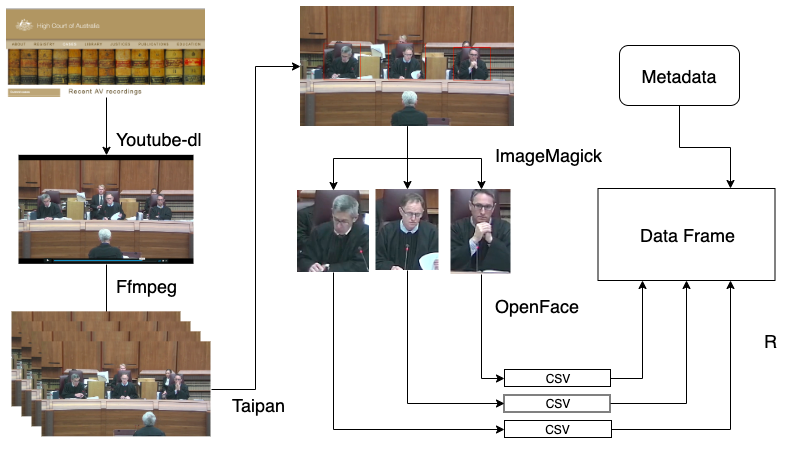
\includegraphics[width=1\linewidth]{figures/workflow} \caption{data processing workflow \label{fig:workflow}}\label{fig:unnamed-chunk-1}
\end{figure}

\hypertarget{variable-description}{%
\section{Variable description}\label{variable-description}}

OpenFace provides more than 711 variables measuring different aspect of a given face and a full description of the output variables can be found \href{https://github.com/TadasBaltrusaitis/OpenFace/wiki/Action-Units}{here}. This outlines the difficulty of this project: no existing models will present accurate prediction and inference using 700+ variables - how can we incorporate these information to say about the facial expressions of the Justices during the hearings?

I conduct some exploratory data analysis on one video: \texttt{Nauru\_a} and find the 700+ variables can be classified as follows with some insights

\begin{itemize}
\item
  \textbf{Confidence}: How confidence OpenFace is with the detection. Confidence is related to the angle that the Justice's face present in the images.
\item
  \textbf{Gaze}: Gaze tracking: the vector from the pupil to corneal reflection. The dataset contains information on the gaze for both eyes while there is no distinct difference between the eyes. Also I was trying to make animation to track the change of the gaze for judges but no good luck.
\item
  \textbf{Pose}: the location of the head with respect to camera. Pose-related variables don't provide much useful information apart from gaze-related variables.
\item
  \textbf{Landmarking}: landmarking variables for face and eyes. Landmarking variables allows me to plot the face of the judge in a particular frame. More work could be done to explore the usefulness of landmarking variables.
\item
  \textbf{Action Unit}: Action units are used to describe facial expressions. \href{https://imotions.com/blog/facial-action-coding-system/}{this website} provides a good animation on each action unit. The action unit has intensity measures ending with \texttt{\_c} and presence measures ending with \texttt{\_r}. These variables will be the focus of my project and a reference study of using action units to detect human emotion by Kovalchik can be found \href{http://www.sloansportsconference.com/wp-content/uploads/2018/02/2005.pdf}{here}.
\end{itemize}

\hypertarget{data-format}{%
\section{Data format}\label{data-format}}

In this project, we will make use of the action unit variables along with all the added indexes to analyse the face of the judge. In the wide format, apart from the first four index columns, each action unit has two columns with one for binary presence value and another for numeric intensity value. The Table \ref{tab:wide} presents the first five rows of the dataset with columns for the first action unit only.

\begin{table}[ht]
\begin{center}
\caption{\label{tab:wide} data in wide format}
\begin{tabular}{lllllllllllllllllllllllllllllllllllllll}
\toprule
judge & video & frame & AU01-r & AU02-r & AU04-r & AU05-r & AU06-r & AU07-r & AU09-r & AU10-r & AU12-r & AU14-r & AU15-r & AU17-r & AU20-r & AU23-r & AU25-r & AU26-r & AU45-r & speaker & AU01-c & AU02-c & AU04-c & AU05-c & AU06-c & AU07-c & AU09-c & AU10-c & AU12-c & AU14-c & AU15-c & AU17-c & AU20-c & AU23-c & AU25-c & AU26-c & AU28-c & AU45-c \\
\midrule
Bell & McKell & 1 & 0 & 0 & 0.69 & 0.63 & 0 & 1.5 & 0 & 0 & 0 & 0 & 0 & 0 & 0.05 & 0 & 0 & 0.26 & 0.47 & Appellent & 0 & 1 & 1 & 0 & 0 & 1 & 1 & 0 & 0 & 0 & 1 & 0 & 1 & 0 & 1 & 0 & 0 & 0 \\
Bell & McKell & 2 & 0 & 0 & 0.69 & 0.63 & 0 & 1.5 & 0 & 0 & 0 & 0 & 0 & 0 & 0.05 & 0 & 0 & 0.26 & 0.47 & Appellent & 1 & 1 & 1 & 1 & 1 & 1 & 1 & 0 & 0 & 1 & 1 & 0 & 1 & 0 & 0 & 0 & 0 & 0 \\
\bottomrule
\end{tabular}
\end{center}
\end{table}

The data can also be expressed in the long format with action unit being another index and presence and intensity being two columns. The Table \ref{tab:long} presents the first five rows of the data in the long format.

\begin{table}[ht]
\begin{center}
\caption{\label{tab:long} data in long format}
\begin{tabular}{lllllll}
\toprule
judge & video & frame & speaker & AU & presence & intensity \\
\midrule
Bell & McKell & 1 & Appellent & AU01 &  1 & 0.00 \\
Bell & McKell & 1 & Appellent & AU02 &  1 & 0.00 \\
Bell & McKell & 1 & Appellent & AU04 &  0 & 0.69 \\
Bell & McKell & 1 & Appellent & AU05 &  1 & 0.63 \\
Bell & McKell & 1 & Appellent & AU06 &  0 & 0.00 \\
Bell & McKell & 1 & Appellent & AU07 &  1 & 1.54 \\
Bell & McKell & 1 & Appellent & AU09 &  1 & 0.00 \\
Bell & McKell & 1 & Appellent & AU10 &  1 & 0.00 \\
Bell & McKell & 1 & Appellent & AU12 &  0 & 0.00 \\
Bell & McKell & 1 & Appellent & AU14 &  0 & 0.00 \\
Bell & McKell & 1 & Appellent & AU15 &  1 & 0.00 \\
Bell & McKell & 1 & Appellent & AU17 &  0 & 0.00 \\
Bell & McKell & 1 & Appellent & AU20 &  1 & 0.05 \\
Bell & McKell & 1 & Appellent & AU23 &  0 & 0.00 \\
Bell & McKell & 1 & Appellent & AU25 &  1 & 0.00 \\
Bell & McKell & 1 & Appellent & AU26 &  0 & 0.26 \\
Bell & McKell & 1 & Appellent & AU28 & NA &   NA \\
Bell & McKell & 1 & Appellent & AU45 &  0 & 0.47 \\
Bell & McKell & 2 & Appellent & AU01 &  0 & 0.00 \\
Bell & McKell & 2 & Appellent & AU02 &  1 & 0.00 \\
Bell & McKell & 2 & Appellent & AU04 &  1 & 0.69 \\
Bell & McKell & 2 & Appellent & AU05 &  1 & 0.63 \\
Bell & McKell & 2 & Appellent & AU06 &  0 & 0.00 \\
Bell & McKell & 2 & Appellent & AU07 &  1 & 1.54 \\
Bell & McKell & 2 & Appellent & AU09 &  1 & 0.00 \\
Bell & McKell & 2 & Appellent & AU10 &  1 & 0.00 \\
Bell & McKell & 2 & Appellent & AU12 &  0 & 0.00 \\
Bell & McKell & 2 & Appellent & AU14 &  0 & 0.00 \\
Bell & McKell & 2 & Appellent & AU15 &  1 & 0.00 \\
Bell & McKell & 2 & Appellent & AU17 &  0 & 0.00 \\
Bell & McKell & 2 & Appellent & AU20 &  1 & 0.05 \\
Bell & McKell & 2 & Appellent & AU23 &  0 & 0.00 \\
Bell & McKell & 2 & Appellent & AU25 &  1 & 0.00 \\
Bell & McKell & 2 & Appellent & AU26 &  0 & 0.26 \\
Bell & McKell & 2 & Appellent & AU28 & NA &   NA \\
Bell & McKell & 2 & Appellent & AU45 &  0 & 0.47 \\
\bottomrule
\end{tabular}
\end{center}
\end{table}

\hypertarget{missing-value-imputation}{%
\section{Missing value imputation}\label{missing-value-imputation}}

The missingness in the dataset could be due to the fact that a judge is reading the materials on the desk so the face is not captured for a particular frame or simply because some faces are not detectable for the given resolution of the video stream. However, since that data is in time series structure, simply drop the missing observation will cause the time interval to be irregular and complicate further analysis.

There are two different sets of variables that need imputation. \texttt{Presence} is a binary variable that takes value of one if an action unit is present in a particular frame for a judge in a video and \texttt{Intensity} measures how strong that action unit is. Linear interpolation from \texttt{forecast} package is suitable to impute \texttt{Intensity} and \texttt{Presence} is imputed through sampling from binomial distribution. The imputed action unit data is stored as \texttt{au\_imputed} under the \texttt{raw\_data} folder.

\hypertarget{data-cleaning}{%
\section{Data cleaning}\label{data-cleaning}}

There is a data quality issue coming from the data I get from OpenFace. For some observations, the intensity of the action unit could be high while the present variable has a zero value. This does not make sense since if an action unit has been detected as strong intensity for a judge in a particular frame, it should at least present on the judge's face. Therefore, I adjust for the presence value if the intensity is higher than one. One is being chosen as the threshold value since in Ekman's definition of the intensity of the action unit, a score of one means the action unit is at least slightly present in the judge's face. The adjusted data is stored as \texttt{au\_tidy} under the \texttt{raw\_data} folder.

\hypertarget{methods}{%
\chapter{Methods}\label{methods}}

Here you need to write about the analytical methods that you are using

\hypertarget{results}{%
\chapter{Results}\label{results}}

\hypertarget{notation}{%
\section{Notation}\label{notation}}

Let \(\mathbf{X}\) be a matrix of predictors, and \(\mathbf{Y}\) variable in our case is bivariate matrix of response variables, including a binary indicator of presence/absence and a numeric value measuring intensity, of facial action unit, where

\begin{itemize}
\tightlist
\item
  \(X_1\) indicates \texttt{judge} with six categories \(i = 1,2, \cdots, 6\)
\item
  \(X_2\) indicates \texttt{video} for each of the seven cases, \(j = 1,2, \cdots, 7\)
\item
  \(X_3\) indicates action unit containing 18 possible facial expression.\\
\item
  \(X_4\) indicates \texttt{speaker}, either the appellant or respondent, \(l=1,2\)
\item
  \(X_5\) indicates \texttt{frame} corresponding to time, \(t = 1,2, \cdots, T_j\)
\end{itemize}

Note that \(t\) could be considered a time variable, but because images are taken at 1 minute intervals, temporal dependence is unlikely to exist. Rather this should be considered an independent observation.

A full, main effects model for the data might be expressed as:

\[Y_{ijkl} = \mu + \alpha_i + \beta_j + \gamma_k + \delta_l + \varepsilon_{ijkl}\]

\noindent and we would be interested in interactions between judge, case, action unit and who is speaking. An alternative model structure, is to treat each action unit individually, and fit separate models.

Also, let \(P_{jitkl}\) represent the response variable presence, and \(I_{jitkl}\) represent the second response variable intensity. This notation will be helpful for defining the plots and models explained in this section.

\hypertarget{action-unit-presence}{%
\section{Action unit: Presence}\label{action-unit-presence}}

\hypertarget{mean-presence}{%
\subsection{Mean presence}\label{mean-presence}}

I first compute the average presence (\(P_{ik}\)) of each action unit for each judge as \[P_{ik} = \frac{\sum_{jt}X_{ijtk}}{\sum_{j = 1}^JT_j}\] This is then plotted in Figure \ref{fig:mean_presence} to give an overview of the presence of all the action units across all the judge. The order of action unit on the y axis is ranked by the average presence of all the judge. The five most frequent action units are highlighted in blue for each judge and summarised in Table \ref{tab:most_common}

\begin{figure}
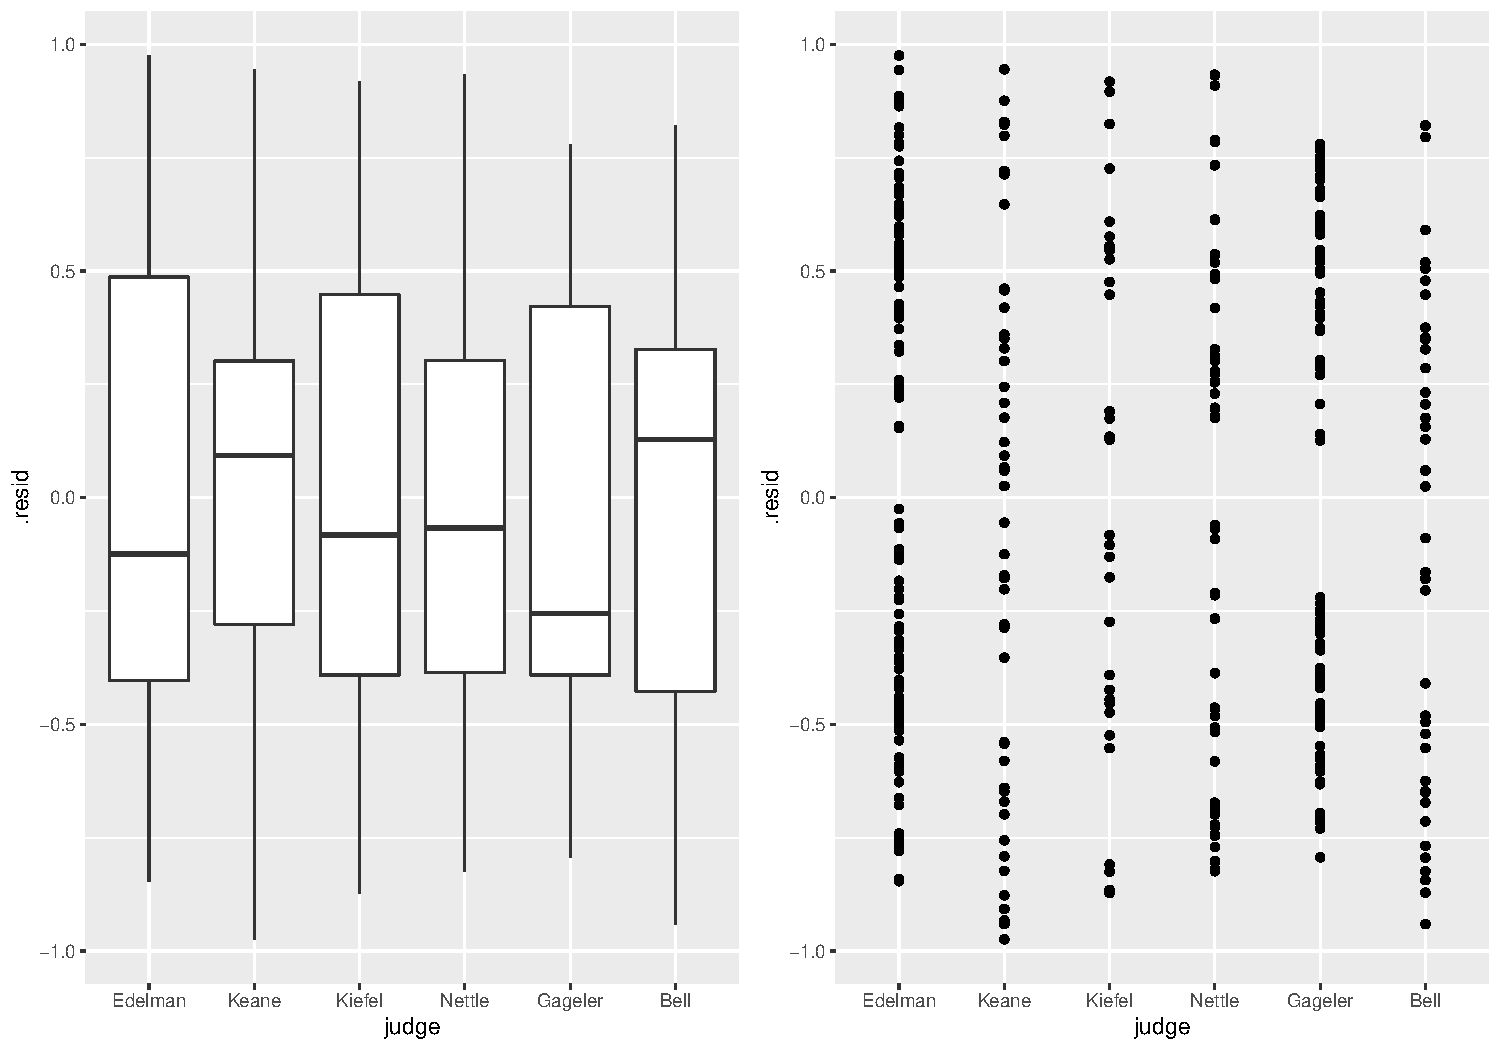
\includegraphics[width=1\linewidth]{thesis_files/figure-latex/unnamed-chunk-4-1} \caption{The average presence score of each action unit for each judge, aggregating on video and time. \label{fig:mean_presence}}\label{fig:unnamed-chunk-4}
\end{figure}

\begin{table}[t]

\caption{\label{tab:unnamed-chunk-5}\label{tab:most_common}The five most commonly presented action unit for each judge.}
\centering
\begin{tabular}{r|l|l|l|l|l|l}
\hline
index & Bell & Edelman & Gageler & Keane & Kiefel & Nettle\\
\hline
1 & AU15 & AU02 & AU02 & AU20 & AU02 & AU02\\
\hline
2 & AU09 & AU20 & AU05 & AU15 & AU25 & AU15\\
\hline
3 & AU25 & AU01 & AU15 & AU02 & AU45 & AU20\\
\hline
4 & AU02 & AU15 & AU14 & AU14 & AU20 & AU01\\
\hline
5 & AU01 & AU23 & AU20 & AU07 & AU14 & AU07\\
\hline
\end{tabular}
\end{table}

It can be seen that some of the action units are common across almost all the judges, these includes

\begin{itemize}
\tightlist
\item
  AU02 (outer eyebrow raise),
\item
  AU20 (lip stretcher),
\item
  AU15 (Lip Corner Depressor)
\item
  AU14 (Dimpler)
\end{itemize}

AU02 makes a contribution to surprise, which is a positive attitude showing that judges are interested in a particular moment \autocite{ekman2002facial}. According to \autocite{ekman2002facial}, AU14 indicates boredom and AU15 shows confusion. Along with other action units that presented with high frequency in a particular judge but not all (summarised in Table \ref{tab:other_highf}), the emotions judges displayed in the courtroom can be summarised into three categories, described in Table \ref{tab:three_category} along with the featured action units.

\begin{table}[t]

\caption{\label{tab:unnamed-chunk-6}\label{tab:three_category} Summarised emotions and featured action units}
\centering
\begin{tabular}{l|l}
\hline
emotion & Featured Action Unit\\
\hline
Surprise & AU01, AU02, AU05\\
\hline
Boredom & AU14, AU23\\
\hline
Confusion & AU07, AU15, AU23\\
\hline
\end{tabular}
\end{table}

\begin{table}[t]

\caption{\label{tab:unnamed-chunk-7}\label{tab:other_highf} Other high frequent action units }
\centering
\begin{tabular}{l|l|l|l}
\hline
judge & first & second & third\\
\hline
Bell & AU09: Nose wrinkler & AU25: Lips part & AU01: Inner brow raiser\\
\hline
Edelman & AU01: Inner brow raiser & AU23: Lip tightener & NA\\
\hline
Gageler & AU05: Upper lid raiser & NA & NA\\
\hline
Keane & AU07: Lid tightener & NA & NA\\
\hline
Kiefel & AU25: Lips part & AU45: Blink & NA\\
\hline
Nettle & AU01: Inner brow raiser & AU07: Lid tightener & NA\\
\hline
\end{tabular}
\end{table}

\hypertarget{model-fit}{%
\subsection{Model fit}\label{model-fit}}

The first model I use is a generalised linear model with binomial link to understand the presence of the action units. The variables used include the judge, action units and their interactions. The use of interaction terms allow for the effect of judge to be differed at different action unit level. The model can be written down as Equation \ref{eq:judge_au}.Judge Edelman and AU01 are selected as the base level.

\begin{equation}\label{eq:judge_au}
P_{ik} = \mu + \alpha_i + \gamma_k + (\alpha\gamma)_{ik}
\end{equation}

I'm interested to know if the presence score for one pair of judge and action unit is signficiantly different from another pair. Aanalysis of Varaince (ANOVA) test result in Table \ref{tab:anova} shows that there are significant variance for both judge, AU and their interactions. The next step after ANOVA is to test how each level of judge and AU different from another and I use multiple comparison to do this. (manually it will be 861 test to perform since 6 judges and 7 au - using multiple comparison, we can perform this take while control for a relatively low 5\% false positive rate). The estimated coefficient for each judge and AU pair is reported in Table \ref{tab:result_1} along with the upper and lower confidence interval bond. The information in the group column is helpful to understand how one particular pair of judge and au is different from another pair. With compact letter display, the pair with the same letter/number are \emph{NOT} significantly different from each other.

This result is also plotted in Figure \ref{fig:model_1_plot}. Insights:

\begin{itemize}
\tightlist
\item
  Individual difference:

  \begin{itemize}
  \item
    Kean and Bell has relatively less AU02: Outer brow raiser presenting
  \item
  \end{itemize}
\end{itemize}

\begin{table}[t]

\caption{\label{tab:anova}\label{tab:anova}ANOVA result}
\centering
\begin{tabular}{l|r|r|r|r}
\hline
  & Df & Deviance & Resid. Df & Resid. Dev\\
\hline
NULL & NA & NA & 15183 & 18900.38\\
\hline
judge & 5 & 298.5383 & 15178 & 18601.84\\
\hline
AU & 3 & 1682.9621 & 15175 & 16918.88\\
\hline
judge:AU & 15 & 1113.8722 & 15160 & 15805.01\\
\hline
\end{tabular}
\end{table}

\begin{table}[ht]
\begin{center}
\caption{\label{tab:result_1} model result}
\begin{tabular}{lllllll}
\toprule
judge & AU & prob & SE & df & asymp.LCL & asymp.UCL \\
\midrule
Edelman & AU02 & 0.95 & 0.0069 & Inf & 0.93 & 0.96 \\
Bell & AU02 & 0.73 & 0.0223 & Inf & 0.68 & 0.77 \\
Gageler & AU02 & 0.85 & 0.0125 & Inf & 0.83 & 0.88 \\
Keane & AU02 & 0.78 & 0.0207 & Inf & 0.74 & 0.82 \\
Kiefel & AU02 & 0.95 & 0.0091 & Inf & 0.93 & 0.97 \\
Nettle & AU02 & 1.00 & 0.0028 & Inf & 0.99 & 1.00 \\
Edelman & AU14 & 0.43 & 0.0155 & Inf & 0.40 & 0.46 \\
Bell & AU14 & 0.15 & 0.0179 & Inf & 0.12 & 0.19 \\
Gageler & AU14 & 0.62 & 0.0173 & Inf & 0.58 & 0.65 \\
Keane & AU14 & 0.71 & 0.0227 & Inf & 0.66 & 0.75 \\
Kiefel & AU14 & 0.52 & 0.0211 & Inf & 0.48 & 0.56 \\
Nettle & AU14 & 0.49 & 0.0201 & Inf & 0.45 & 0.52 \\
Edelman & AU15 & 0.46 & 0.0156 & Inf & 0.43 & 0.49 \\
Bell & AU15 & 0.86 & 0.0176 & Inf & 0.82 & 0.89 \\
Gageler & AU15 & 0.62 & 0.0172 & Inf & 0.59 & 0.66 \\
Keane & AU15 & 0.87 & 0.0170 & Inf & 0.83 & 0.90 \\
Kiefel & AU15 & 0.44 & 0.0210 & Inf & 0.40 & 0.48 \\
Nettle & AU15 & 0.78 & 0.0166 & Inf & 0.75 & 0.81 \\
Edelman & AU20 & 0.77 & 0.0132 & Inf & 0.74 & 0.79 \\
Bell & AU20 & 0.62 & 0.0242 & Inf & 0.57 & 0.67 \\
Gageler & AU20 & 0.55 & 0.0177 & Inf & 0.51 & 0.58 \\
Keane & AU20 & 0.93 & 0.0131 & Inf & 0.90 & 0.95 \\
Kiefel & AU20 & 0.84 & 0.0154 & Inf & 0.81 & 0.87 \\
Nettle & AU20 & 0.74 & 0.0176 & Inf & 0.71 & 0.77 \\
\bottomrule
\end{tabular}
\end{center}
\end{table}

\begin{figure}
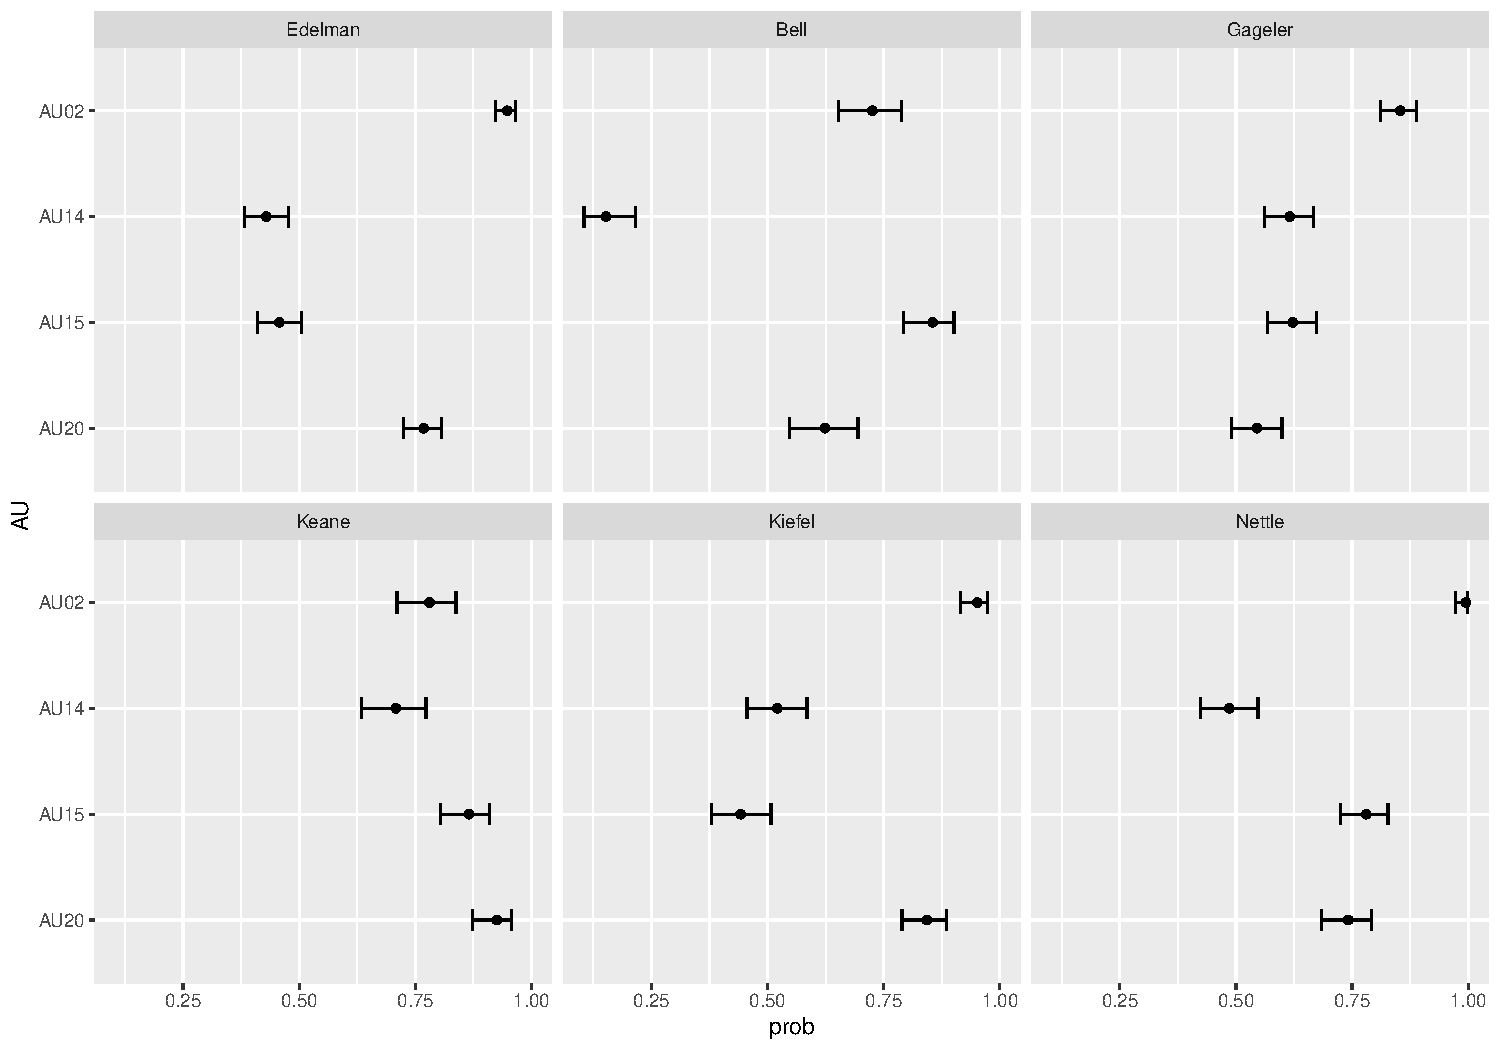
\includegraphics[width=1\linewidth]{thesis_files/figure-latex/unnamed-chunk-9-1} \caption{THis is the graphical representation of model1\label{fig:model_1_plot}}\label{fig:unnamed-chunk-9}
\end{figure}

\hypertarget{presence-by-videos}{%
\subsection{Presence by videos}\label{presence-by-videos}}

Apart from visualising the general presence score for all the action units, I'm also interested in the break down statistics by video (\(P_{ijk}\)). This is computed as \[P_{ijk} = \frac{\sum_{t}X_{ijtk}}{T_j}\] for the four most common action units: AU02, AU14, AU15, AU20 and plotted in Figure \ref{fig:common_video}. From this plot, we can observe that

\begin{itemize}
\item
  some of the judge are have relatively stable display of action unit throughout different videos (i.e.~Edelman and Nettle),
\item
  while Gagaler seems to be highly reactive to some cases (i.e.~OKS, Nauru\_a, Nauru\_b).
\end{itemize}

\begin{figure}
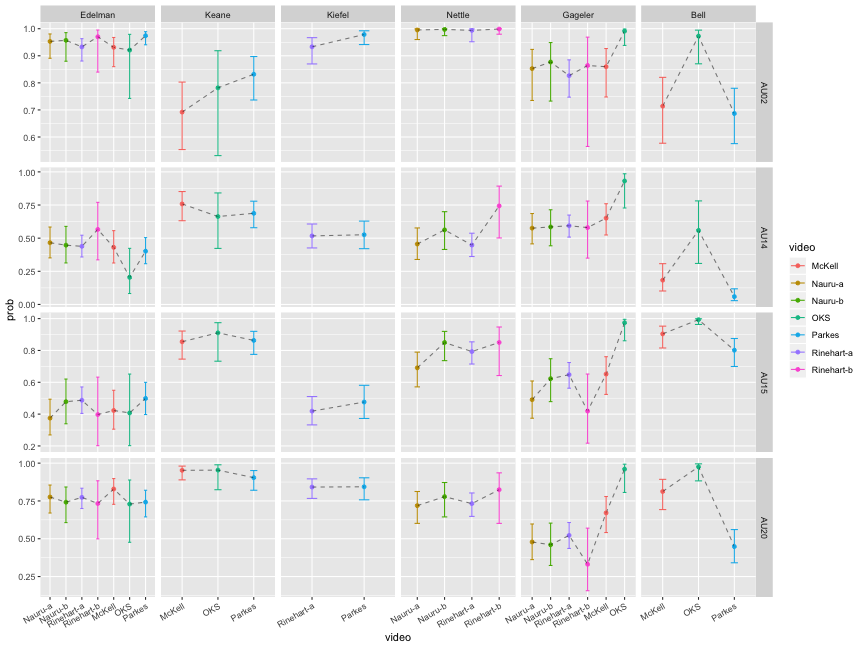
\includegraphics[width=1\linewidth]{thesis_files/figure-latex/unnamed-chunk-10-1} \caption{Average presence of the four most common action units for each judge by video\label{fig:common_video}}\label{fig:unnamed-chunk-10}
\end{figure}

\hypertarget{model-fit-1}{%
\subsection{Model fit}\label{model-fit-1}}

The second model as shown in Equation \ref{eq:judge_video} is estimated to understand the interaction effect between judge and video while taking into account the main effect of judge, video and action unit and other pair wise interactions.

\begin{equation}\label{eq:judge_video}
P_{ijk} = \mu + \alpha_i + \beta_j +\gamma_k + (\alpha\beta)_{ij} + (\alpha\gamma)_{ik} + (\beta\gamma)+{jk}
\end{equation}

Building upon the previous model, we incorporate the effect of videos in this model. There are three main effects of judge, video and action unit in the model. We also incorporate the interaction term between judge and video, which allows the effect of judge to change at each video level. The interaciton term for video and action unit is also added because this allows different videos to have different present score for each different action unit.

The estimated coefficients are presented in Table \ref{tab:result_2}

What we could find from Figure \ref{fig:model_2_plot}

\begin{itemize}
\item
  Judge Edelman, Keane and Kiefel behave relatively consistent throughout all the videos. Judge Gageler is also consistent throughout the trails except for video OKS.
\item
  The interval band for Gageler in case OKS is very different from those in other videos - consistent with exploratory data analysis
\item
  Judge Bell behaves quite differently in the three videos she participates - consistent with EDA
\item
  Judge Edelman has one in OKS for AU14 being pretty different -\textgreater{} consistent with EDA
\end{itemize}

\begin{figure}
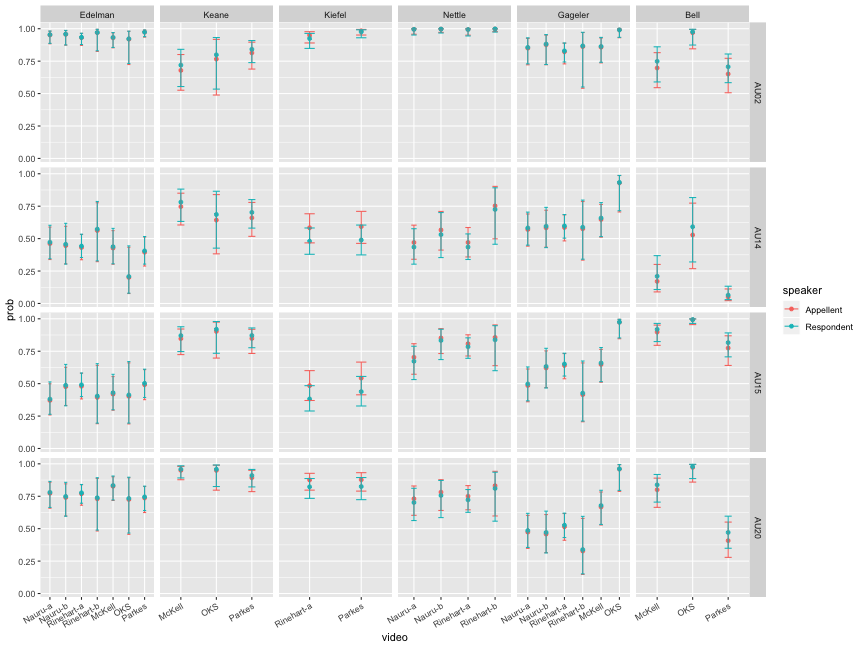
\includegraphics[width=1\linewidth]{thesis_files/figure-latex/unnamed-chunk-11-1} \caption{This is the graphical representaion for model 2\label{fig:model_2_plot}}\label{fig:unnamed-chunk-11}
\end{figure}

\hypertarget{appellant-vs.respondent}{%
\subsection{Appellant vs.~Respondent}\label{appellant-vs.respondent}}

The third model as shown in Equation \ref{eq:judge_speaker} is estimated to understand the interaction effect between judge and speaking party.

\begin{equation}\label{eq:judge_speaker}
P_{ijk} = \mu + \alpha_i + \beta_j +\gamma_k + \delta_l + (\alpha\delta)_{il}
\end{equation}

The estimated coefficients are presented in Table \ref{tab:result_3}

What we could find from Figure \ref{fig:model_3_plot}

\begin{itemize}
\tightlist
\item
  Judges are behaving pretty similar when different parties are talking
\end{itemize}

\begin{figure}
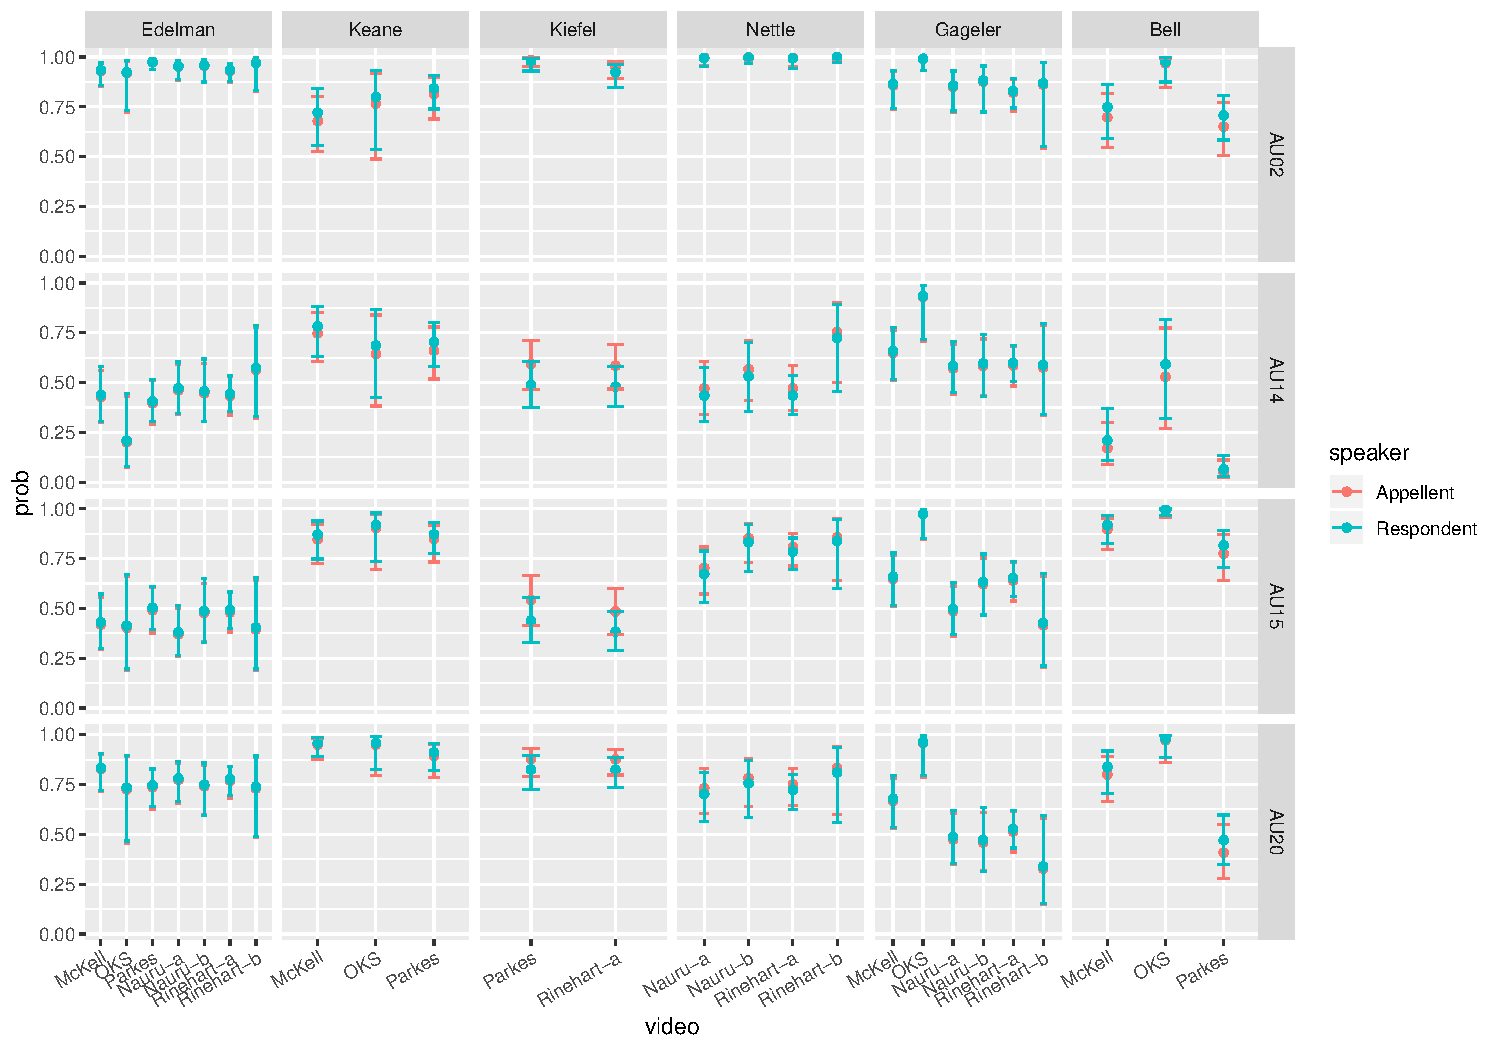
\includegraphics[width=1\linewidth]{thesis_files/figure-latex/unnamed-chunk-13-1} \caption{THis is the graphical representation of model3\label{fig:model_3_plot}}\label{fig:unnamed-chunk-13}
\end{figure}

\hypertarget{action-unit-intensity}{%
\section{Action unit: Intensity}\label{action-unit-intensity}}

\hypertarget{general-intensity-plot}{%
\subsection{General Intensity plot}\label{general-intensity-plot}}

In Ekman's 20002 FACS manual, the intensity of an action unit is defined based on five classes: Trace: 0-1, Slight: 1-2, Marked or pronounced: 2-3, Severe or extreme: 3-4 and Maximum: 4-5.

The boxplot of the intensity for all the judges across all the videos is presented in Figure \ref{fig:intensity}. Each bar-and-whisker represents the intensity (\(I_{ijtk}\)) of all the action units aggregated on time for a particular judge \(i\) in a specific case \(j\). For example, the first bar-and-whisker in case Nauru\_a is created using all the 17 action units of Edelman through out the elapsed time in Nauru\_a case.

From the plot, we can see that most of the action units have low intensity score and this is expected because usually judges are expected to behave neutral in the court room. Thus a square root transformation is taken on the y axis for better visualisation effect. We can find that Judge Nettle seems to have higher average in all the four cases he appears: Nauru\_a\&b, Rinehart\_a \&b.

\begin{figure}
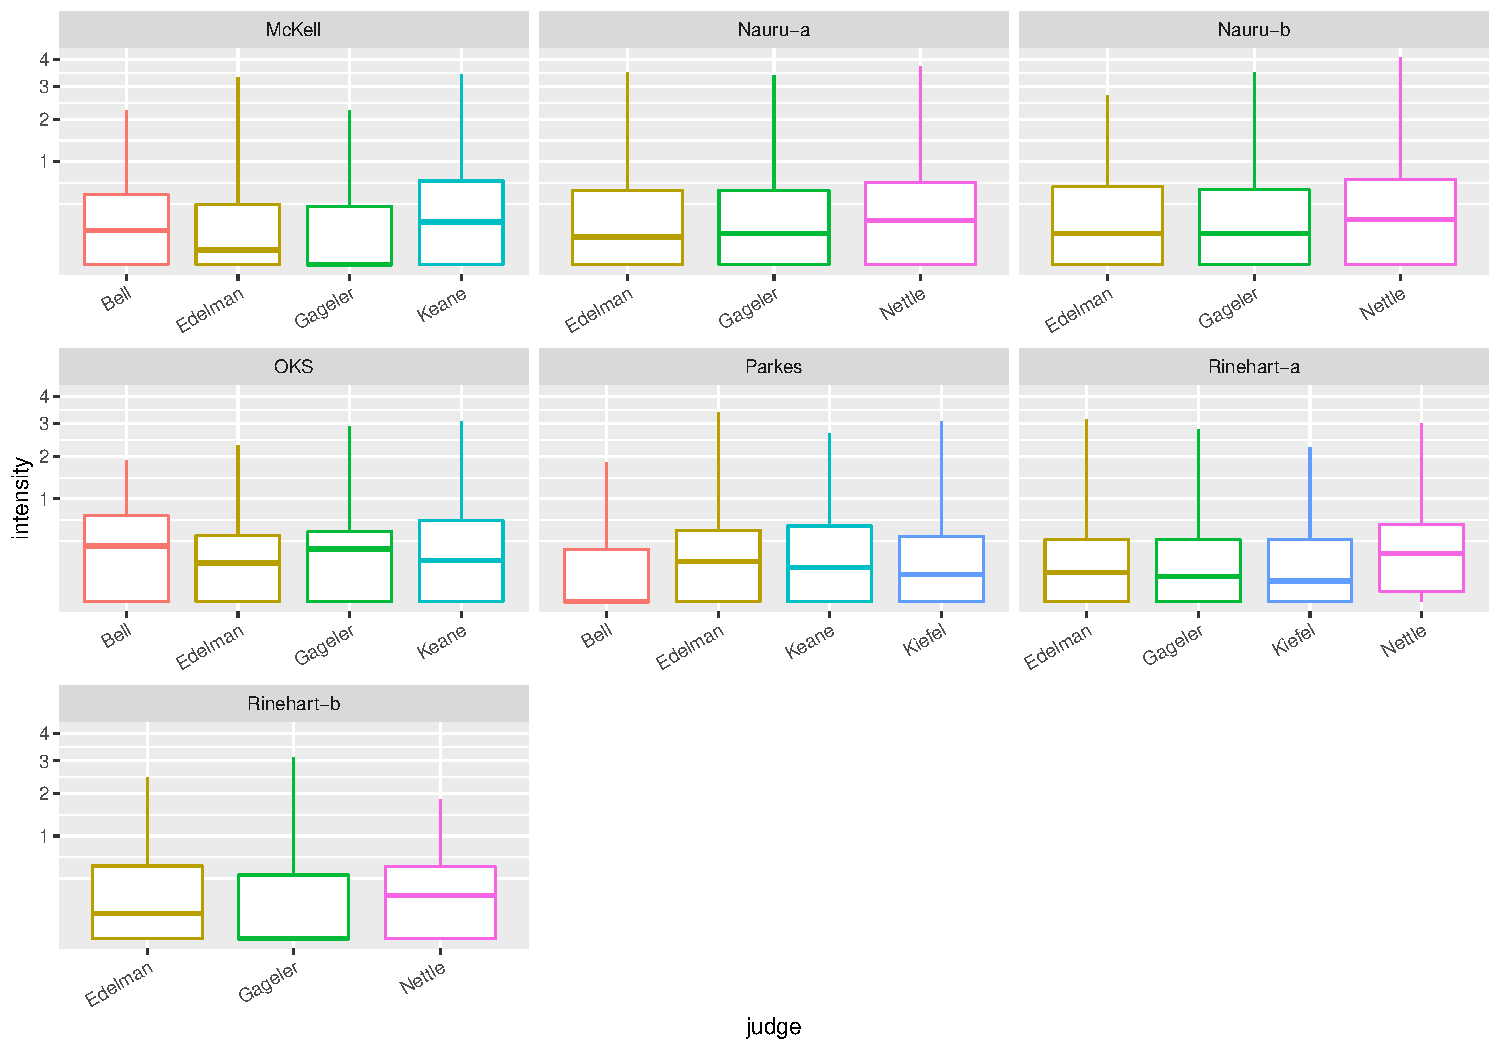
\includegraphics[width=1\linewidth]{thesis_files/figure-latex/unnamed-chunk-14-1} \caption{General intensity score by judge and video\label{fig:intensity}}\label{fig:unnamed-chunk-14}
\end{figure}

\hypertarget{mean-intensity}{%
\subsection{Mean intensity}\label{mean-intensity}}

Mean intensity score (\(I_{ik}\)) of each action unit for each of the judge is computed as \[I_{ik} = \frac{\sum_{jt}X_{ijtk}}{\sum_{j = 1}^JT_j}\] and plotted in Figure \ref{fig:mean_intensity}. The five most intense action units for each judge are presented in Table \ref{tab:most_intense}. We can find that the common high intense action units includes

\begin{itemize}
\tightlist
\item
  AU20 (Lip Stretcher)
\item
  AU07 (Lid Tightener)
\item
  AU04 (Brow Lowerer)
\end{itemize}

AU04 also belongs to the confusion category as AU07. This could help to understand that judges are more likely to express a stronger confusing expression than other emotions.

\begin{figure}
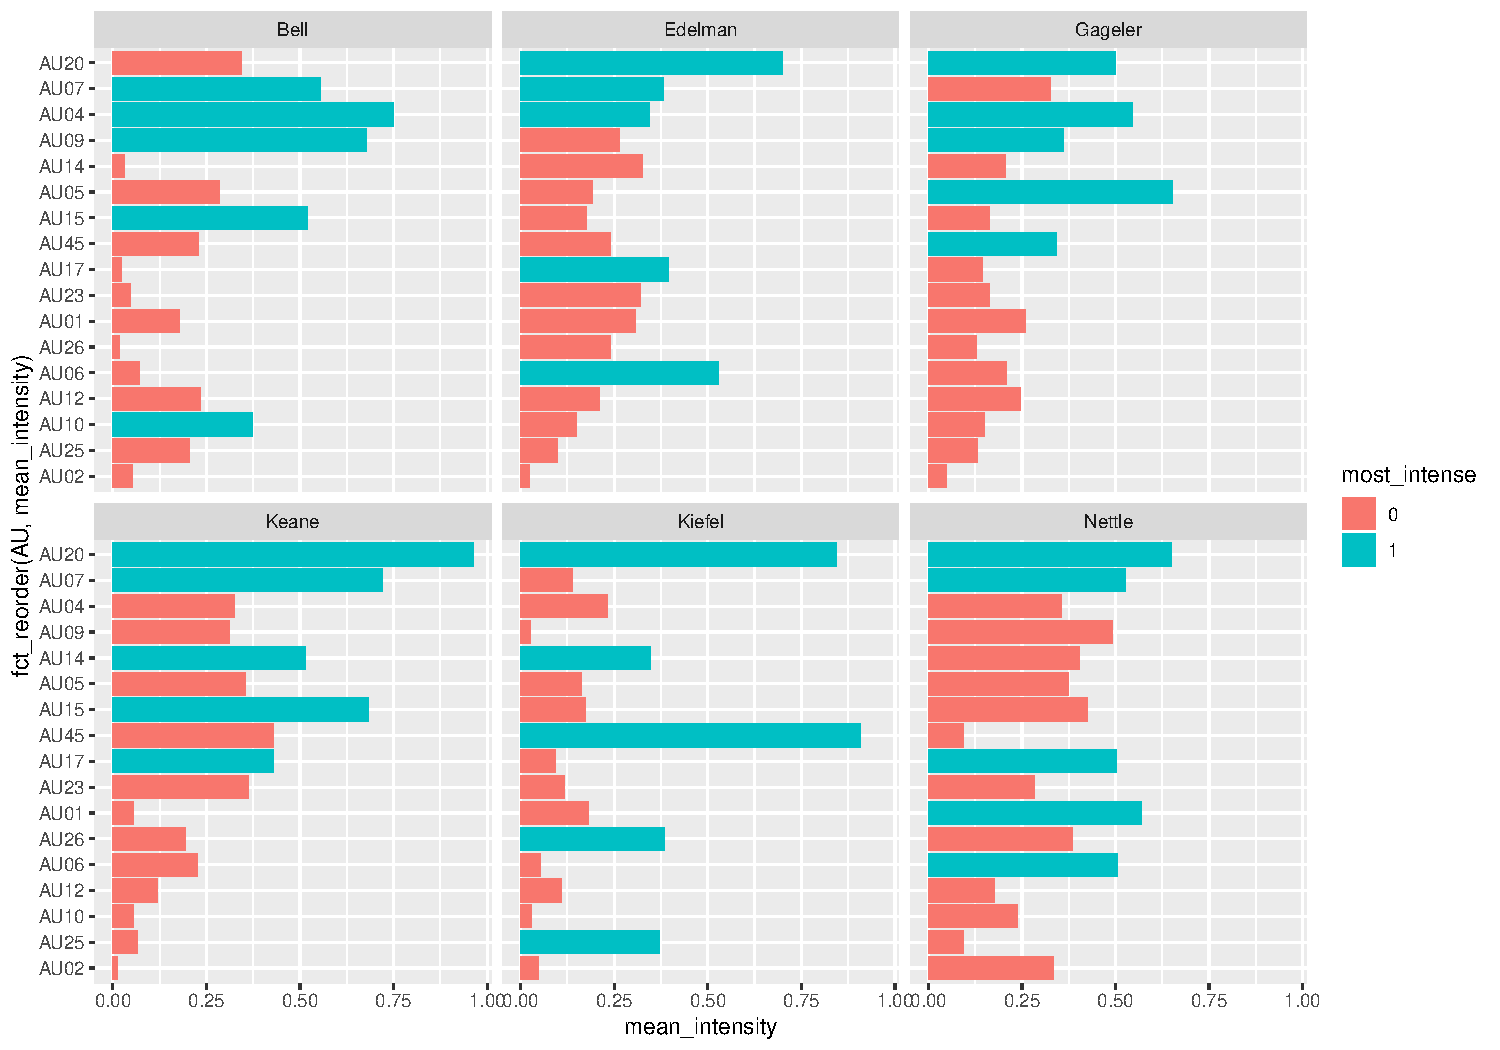
\includegraphics[width=1\linewidth]{thesis_files/figure-latex/unnamed-chunk-16-1} \caption{Mean intensity score for each judge and action unit aggregating on videos.\label{fig:mean_intensity}}\label{fig:unnamed-chunk-16}
\end{figure}

\begin{table}[t]

\caption{\label{tab:unnamed-chunk-17}\label{tab:most_intense}The five most intense action unit for each judge.}
\centering
\begin{tabular}{r|l|l|l|l|l|l}
\hline
index & Bell & Edelman & Gageler & Keane & Kiefel & Nettle\\
\hline
1 & AU04 & AU20 & AU05 & AU20 & AU45 & AU20\\
\hline
2 & AU09 & AU06 & AU04 & AU07 & AU20 & AU01\\
\hline
3 & AU07 & AU17 & AU20 & AU15 & AU26 & AU07\\
\hline
4 & AU15 & AU07 & AU09 & AU14 & AU25 & AU06\\
\hline
5 & AU10 & AU04 & AU45 & AU17 & AU14 & AU17\\
\hline
\end{tabular}
\end{table}

\hypertarget{model-fit-2}{%
\subsection{Model fit}\label{model-fit-2}}

\hypertarget{intensity-plot-for-the-most-frequent-action-units}{%
\subsection{Intensity plot for the most frequent action units}\label{intensity-plot-for-the-most-frequent-action-units}}

Apart from visualising the general intensity score for all the action units, I'm also interested in the intensity score of the most frequent action units. Figure \ref{fig:intensity_by_au} presents this. The statistics being plotted is \(I_{ijtk}\) with \(k\) including AU02, AU14, AU15 and AU20 as the most common four action units. From this plot, we can learn that AU02, although being commonly detected for all the judges, has low intensity score.

\begin{figure}
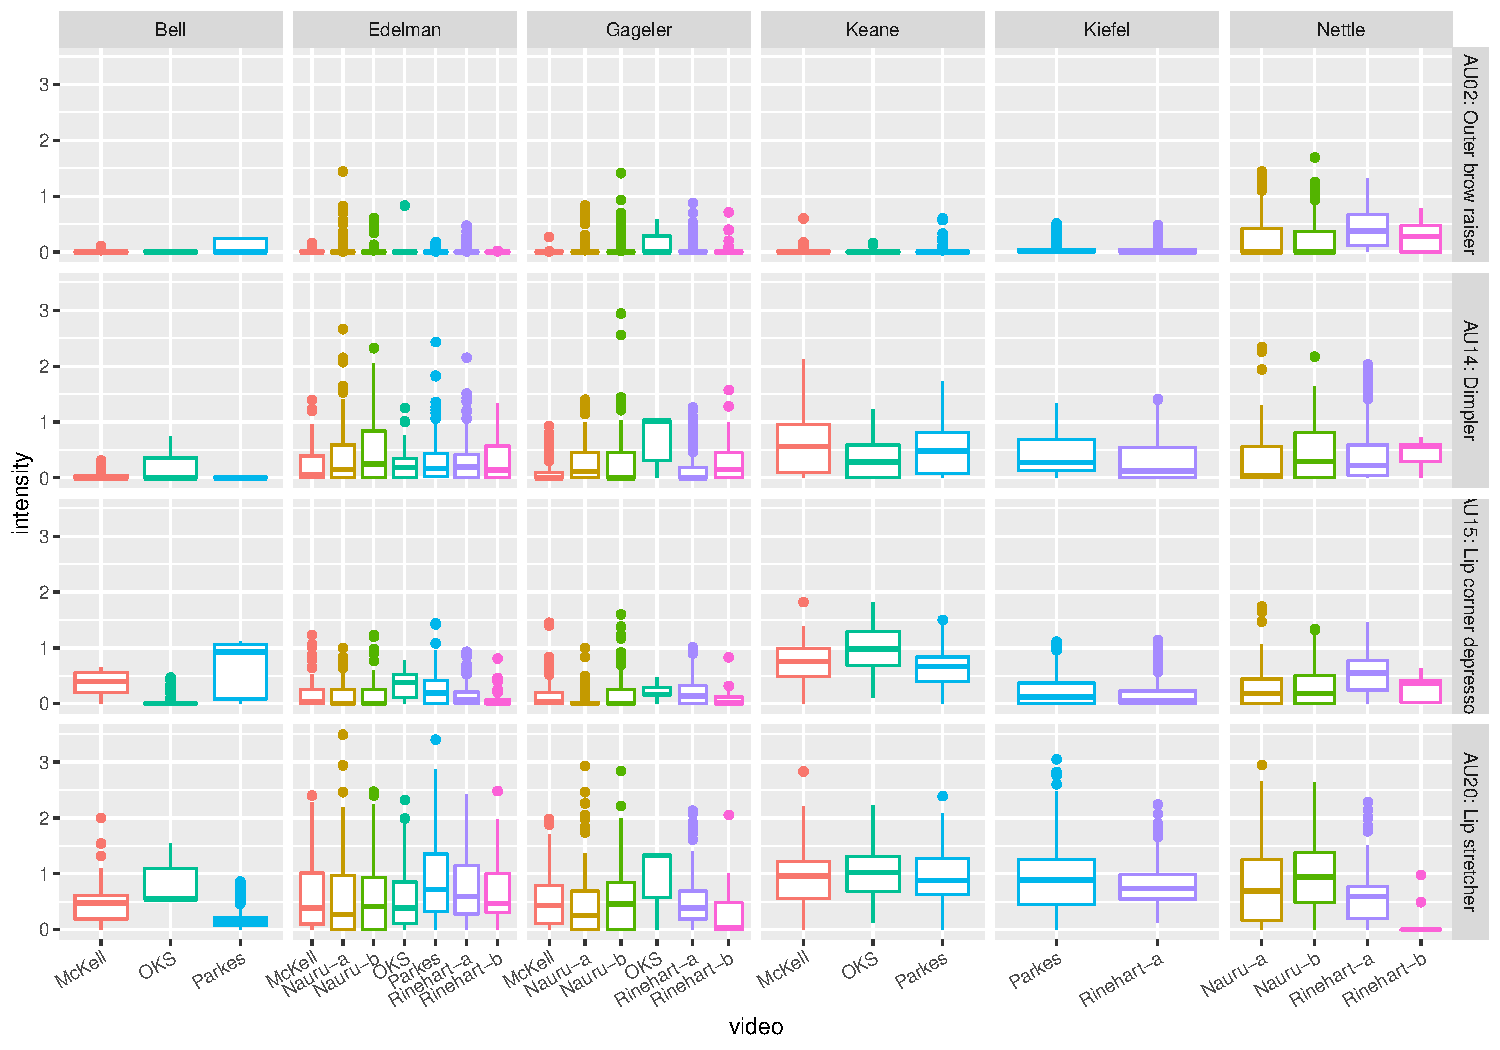
\includegraphics[width=1\linewidth]{thesis_files/figure-latex/unnamed-chunk-19-1} \caption{Intensity score of the most frequent action units, seperating by judge and video ID.\label{fig:intensity_by_au}}\label{fig:unnamed-chunk-19}
\end{figure}

\hypertarget{high-intensity-points}{%
\subsection{High intensity points}\label{high-intensity-points}}

We filter out the points have intensity greater than 2 (at least ``slight'' as per Ekman) in the previous plot and plot it against time and color by the speaker. It tells us that Edelman, Gageler and Nettle are the judges have stronger emotion that can be detected (since they have more points with intensity greater than 2). Different judges also have different time where they display stronger emotions. For example, Justice Nettle are more likely to have stronger emotion throughout the time when the appellant is speaking but only at the beginning and ending period when the respondent is speaking.

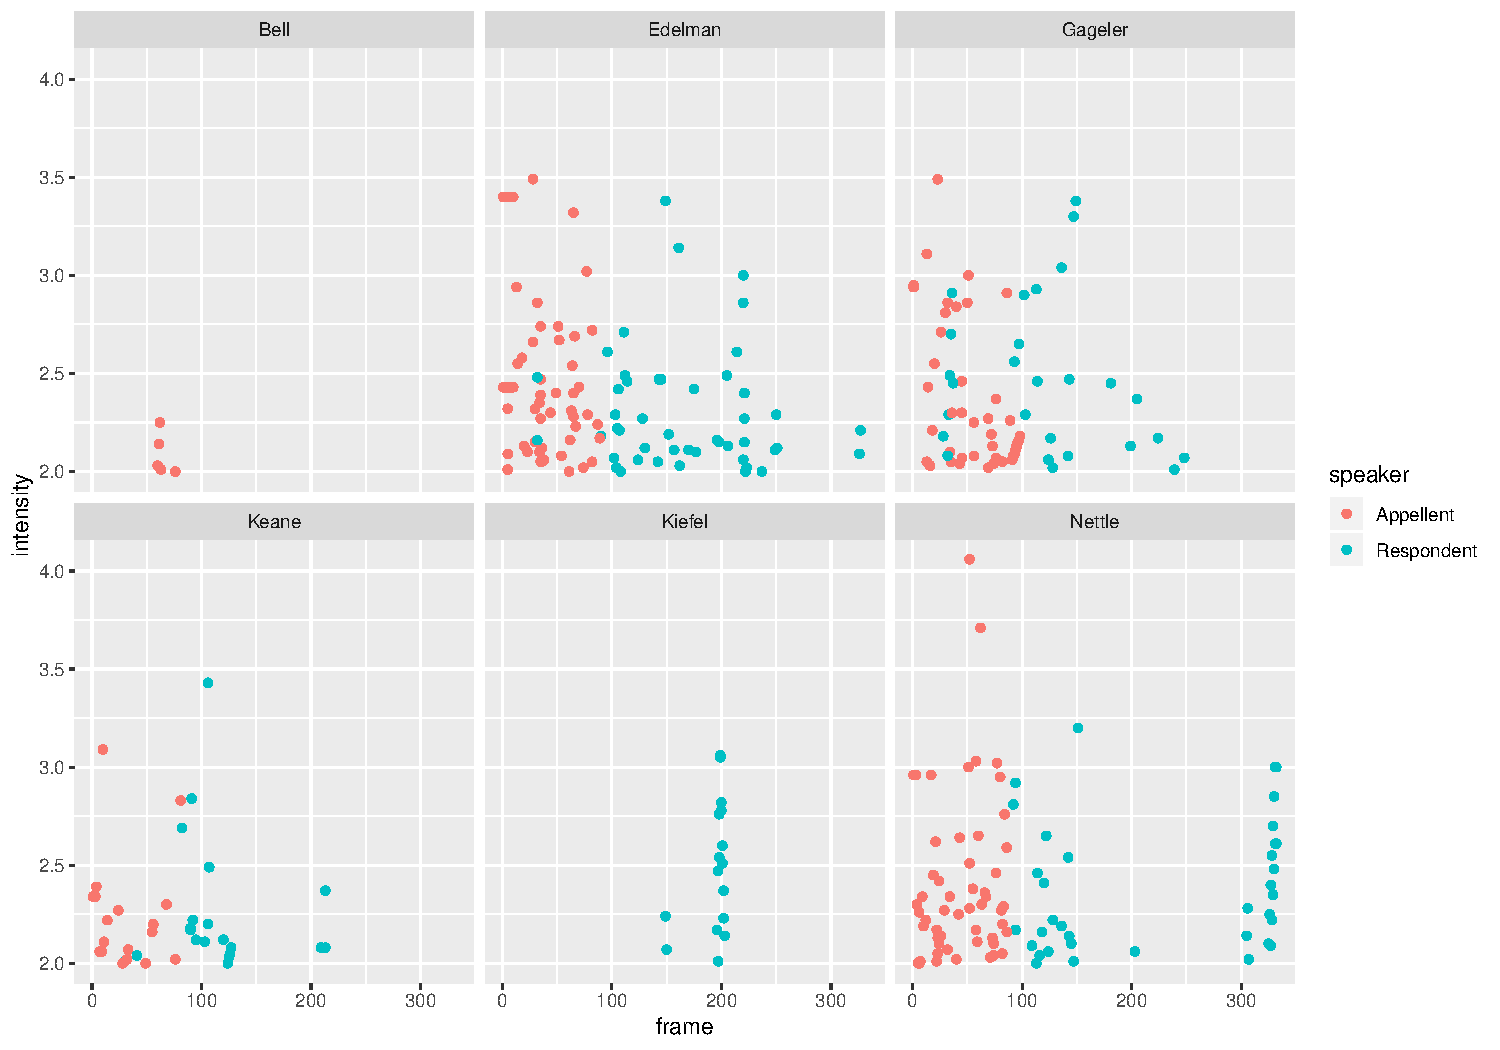
\includegraphics[width=1\linewidth]{thesis_files/figure-latex/unnamed-chunk-20-1}

\appendix

\hypertarget{additional-stuff}{%
\chapter{Additional stuff}\label{additional-stuff}}

\begin{longtable}[]{@{}lll@{}}
\caption{Details of videos processed.}\tabularnewline
\toprule
\begin{minipage}[b]{0.42\columnwidth}\raggedright
Case\strut
\end{minipage} & \begin{minipage}[b]{0.14\columnwidth}\raggedright
Name\strut
\end{minipage} & \begin{minipage}[b]{0.35\columnwidth}\raggedright
AV recording link\strut
\end{minipage}\tabularnewline
\midrule
\endfirsthead
\toprule
\begin{minipage}[b]{0.42\columnwidth}\raggedright
Case\strut
\end{minipage} & \begin{minipage}[b]{0.14\columnwidth}\raggedright
Name\strut
\end{minipage} & \begin{minipage}[b]{0.35\columnwidth}\raggedright
AV recording link\strut
\end{minipage}\tabularnewline
\midrule
\endhead
\begin{minipage}[t]{0.42\columnwidth}\raggedright
Republic of Nauru v. WET040\strut
\end{minipage} & \begin{minipage}[t]{0.14\columnwidth}\raggedright
\texttt{Nauru\_a}\strut
\end{minipage} & \begin{minipage}[t]{0.35\columnwidth}\raggedright
\url{http://www.hcourt.gov.au/cases/cases-av/av-2018-11-07a}\strut
\end{minipage}\tabularnewline
\begin{minipage}[t]{0.42\columnwidth}\raggedright
TTY167 v. Republic of Nauru\strut
\end{minipage} & \begin{minipage}[t]{0.14\columnwidth}\raggedright
\texttt{Nauru\_b}\strut
\end{minipage} & \begin{minipage}[t]{0.35\columnwidth}\raggedright
\url{http://www.hcourt.gov.au/cases/cases-av/av-2018-11-07b}\strut
\end{minipage}\tabularnewline
\begin{minipage}[t]{0.42\columnwidth}\raggedright
Rinehart \& Anor v. Hancock Prospecting Pty Ltd \& Ors on 13 Nov 18\strut
\end{minipage} & \begin{minipage}[t]{0.14\columnwidth}\raggedright
\texttt{Rinehart\_a}\strut
\end{minipage} & \begin{minipage}[t]{0.35\columnwidth}\raggedright
\url{http://www.hcourt.gov.au/cases/cases-av/av-2018-11-13}\strut
\end{minipage}\tabularnewline
\begin{minipage}[t]{0.42\columnwidth}\raggedright
Rinehart \& Anor v. Hancock Prospecting Pty Ltd \& Ors on 14 Nov 18\strut
\end{minipage} & \begin{minipage}[t]{0.14\columnwidth}\raggedright
\texttt{Rinehart\_b}\strut
\end{minipage} & \begin{minipage}[t]{0.35\columnwidth}\raggedright
\url{http://www.hcourt.gov.au/cases/cases-av/av-2018-11-14a}\strut
\end{minipage}\tabularnewline
\begin{minipage}[t]{0.42\columnwidth}\raggedright
Parkes Shire Council v. South West Helicopters Pty Limited\strut
\end{minipage} & \begin{minipage}[t]{0.14\columnwidth}\raggedright
\texttt{Parkes}\strut
\end{minipage} & \begin{minipage}[t]{0.35\columnwidth}\raggedright
\url{http://www.hcourt.gov.au/cases/cases-av/av-2018-11-14b}\strut
\end{minipage}\tabularnewline
\begin{minipage}[t]{0.42\columnwidth}\raggedright
McKell v. The Queen\strut
\end{minipage} & \begin{minipage}[t]{0.14\columnwidth}\raggedright
\texttt{McKell}\strut
\end{minipage} & \begin{minipage}[t]{0.35\columnwidth}\raggedright
\url{http://www.hcourt.gov.au/cases/cases-av/av-2018-12-07}\strut
\end{minipage}\tabularnewline
\begin{minipage}[t]{0.42\columnwidth}\raggedright
OKS v. The State of Western Australia\strut
\end{minipage} & \begin{minipage}[t]{0.14\columnwidth}\raggedright
\texttt{OKS}\strut
\end{minipage} & \begin{minipage}[t]{0.35\columnwidth}\raggedright
\url{http://www.hcourt.gov.au/cases/cases-av/av-2019-02-14}\strut
\end{minipage}\tabularnewline
\bottomrule
\end{longtable}

\hypertarget{list-of-the-name-of-ction-units}{%
\section{List of the name of ction units}\label{list-of-the-name-of-ction-units}}

\begin{table}[ht]
\begin{center}
\caption{\label{tab:au_meaning} The meaning of all the action unit estimated}
\begin{tabular}{l}
\toprule
AU-meaning \\
\midrule
AU01: Inner brow raiser \\
AU02: Outer brow raiser \\
AU04: Brow lowerer \\
AU05: Upper lid raiser \\
AU06: Cheek raiser \\
AU07: Lid tightener \\
AU09: Nose wrinkler \\
AU10: Upper lip raiser \\
AU12: Lip corner puller \\
AU14: Dimpler \\
AU15: Lip corner depressor \\
AU17: Chin raiser \\
AU20: Lip stretcher \\
AU23: Lip tightener \\
AU25: Lips part \\
AU26: Jaw drop \\
AU28: Lip suck \\
AU45: Blink \\
\bottomrule
\end{tabular}
\end{center}
\end{table}

\hypertarget{model-estimation-result}{%
\section{Model estimation result}\label{model-estimation-result}}

\begin{center}
\begin{longtable}{lllllll}
\caption{\label{tab:result_2} model result 2}\\
\toprule
judge & video & AU & prob & SE & asymp.LCL & asymp.UCL \\
\midrule
\endhead
\bottomrule
\endfoot
Edelman & McKell & AU02 & 0.931 & 0.01401 & 0.90 & 0.954 \\
Bell & McKell & AU02 & 0.714 & 0.03411 & 0.64 & 0.776 \\
Gageler & McKell & AU02 & 0.860 & 0.02419 & 0.81 & 0.901 \\
Keane & McKell & AU02 & 0.692 & 0.03503 & 0.62 & 0.756 \\
Edelman & Nauru-a & AU02 & 0.953 & 0.01127 & 0.93 & 0.971 \\
Gageler & Nauru-a & AU02 & 0.853 & 0.02556 & 0.80 & 0.896 \\
Nettle & Nauru-a & AU02 & 0.995 & 0.00275 & 0.99 & 0.999 \\
Edelman & Nauru-b & AU02 & 0.957 & 0.01263 & 0.92 & 0.976 \\
Gageler & Nauru-b & AU02 & 0.877 & 0.02850 & 0.81 & 0.923 \\
Nettle & Nauru-b & AU02 & 0.998 & 0.00161 & 0.99 & 0.999 \\
Edelman & OKS & AU02 & 0.921 & 0.02810 & 0.85 & 0.961 \\
Bell & OKS & AU02 & 0.973 & 0.01224 & 0.94 & 0.989 \\
Gageler & OKS & AU02 & 0.991 & 0.00482 & 0.97 & 0.997 \\
Keane & OKS & AU02 & 0.782 & 0.05426 & 0.66 & 0.870 \\
Edelman & Parkes & AU02 & 0.974 & 0.00603 & 0.96 & 0.984 \\
Bell & Parkes & AU02 & 0.687 & 0.02858 & 0.63 & 0.740 \\
Keane & Parkes & AU02 & 0.832 & 0.02202 & 0.78 & 0.871 \\
Kiefel & Parkes & AU02 & 0.979 & 0.00604 & 0.96 & 0.988 \\
Edelman & Rinehart-a & AU02 & 0.933 & 0.01095 & 0.91 & 0.951 \\
Gageler & Rinehart-a & AU02 & 0.827 & 0.01894 & 0.79 & 0.861 \\
Kiefel & Rinehart-a & AU02 & 0.933 & 0.01271 & 0.90 & 0.954 \\
Nettle & Rinehart-a & AU02 & 0.994 & 0.00353 & 0.98 & 0.998 \\
Edelman & Rinehart-b & AU02 & 0.970 & 0.01455 & 0.92 & 0.989 \\
Gageler & Rinehart-b & AU02 & 0.864 & 0.05155 & 0.73 & 0.938 \\
Nettle & Rinehart-b & AU02 & 0.999 & 0.00095 & 0.99 & 1.000 \\
Edelman & McKell & AU14 & 0.431 & 0.03440 & 0.36 & 0.499 \\
Bell & McKell & AU14 & 0.183 & 0.02830 & 0.13 & 0.245 \\
Gageler & McKell & AU14 & 0.651 & 0.03312 & 0.58 & 0.713 \\
Keane & McKell & AU14 & 0.758 & 0.03063 & 0.69 & 0.813 \\
Edelman & Nauru-a & AU14 & 0.466 & 0.03275 & 0.40 & 0.530 \\
Gageler & Nauru-a & AU14 & 0.575 & 0.03218 & 0.51 & 0.637 \\
Nettle & Nauru-a & AU14 & 0.456 & 0.03350 & 0.39 & 0.522 \\
Edelman & Nauru-b & AU14 & 0.447 & 0.03911 & 0.37 & 0.524 \\
Gageler & Nauru-b & AU14 & 0.585 & 0.03848 & 0.51 & 0.658 \\
Nettle & Nauru-b & AU14 & 0.562 & 0.04047 & 0.48 & 0.640 \\
Edelman & OKS & AU14 & 0.204 & 0.04718 & 0.13 & 0.312 \\
Bell & OKS & AU14 & 0.558 & 0.07074 & 0.42 & 0.689 \\
Gageler & OKS & AU14 & 0.931 & 0.02873 & 0.85 & 0.970 \\
Keane & OKS & AU14 & 0.663 & 0.06109 & 0.54 & 0.771 \\
Edelman & Parkes & AU14 & 0.402 & 0.02753 & 0.35 & 0.457 \\
Bell & Parkes & AU14 & 0.059 & 0.01160 & 0.04 & 0.086 \\
Keane & Parkes & AU14 & 0.687 & 0.02796 & 0.63 & 0.740 \\
Kiefel & Parkes & AU14 & 0.526 & 0.02919 & 0.47 & 0.582 \\
Edelman & Rinehart-a & AU14 & 0.438 & 0.02287 & 0.39 & 0.484 \\
Gageler & Rinehart-a & AU14 & 0.594 & 0.02316 & 0.55 & 0.638 \\
Kiefel & Rinehart-a & AU14 & 0.517 & 0.02524 & 0.47 & 0.566 \\
Nettle & Rinehart-a & AU14 & 0.448 & 0.02456 & 0.40 & 0.496 \\
Edelman & Rinehart-b & AU14 & 0.566 & 0.06411 & 0.44 & 0.685 \\
Gageler & Rinehart-b & AU14 & 0.580 & 0.06352 & 0.45 & 0.697 \\
Nettle & Rinehart-b & AU14 & 0.743 & 0.05574 & 0.62 & 0.837 \\
Edelman & McKell & AU15 & 0.423 & 0.03445 & 0.36 & 0.491 \\
Bell & McKell & AU15 & 0.904 & 0.01816 & 0.86 & 0.934 \\
Gageler & McKell & AU15 & 0.652 & 0.03329 & 0.58 & 0.714 \\
Keane & McKell & AU15 & 0.855 & 0.02392 & 0.80 & 0.896 \\
Edelman & Nauru-a & AU15 & 0.375 & 0.03152 & 0.32 & 0.438 \\
Gageler & Nauru-a & AU15 & 0.491 & 0.03294 & 0.43 & 0.555 \\
Nettle & Nauru-a & AU15 & 0.691 & 0.03057 & 0.63 & 0.747 \\
Edelman & Nauru-b & AU15 & 0.478 & 0.03990 & 0.40 & 0.556 \\
Gageler & Nauru-b & AU15 & 0.623 & 0.03813 & 0.55 & 0.694 \\
Nettle & Nauru-b & AU15 & 0.850 & 0.02498 & 0.79 & 0.892 \\
Edelman & OKS & AU15 & 0.407 & 0.06677 & 0.29 & 0.542 \\
Bell & OKS & AU15 & 0.993 & 0.00319 & 0.98 & 0.997 \\
Gageler & OKS & AU15 & 0.974 & 0.01259 & 0.93 & 0.990 \\
Keane & OKS & AU15 & 0.911 & 0.02957 & 0.83 & 0.954 \\
Edelman & Parkes & AU15 & 0.498 & 0.02836 & 0.44 & 0.554 \\
Bell & Parkes & AU15 & 0.801 & 0.02427 & 0.75 & 0.845 \\
Keane & Parkes & AU15 & 0.863 & 0.01969 & 0.82 & 0.897 \\
Kiefel & Parkes & AU15 & 0.476 & 0.02923 & 0.42 & 0.533 \\
Edelman & Rinehart-a & AU15 & 0.487 & 0.02319 & 0.44 & 0.533 \\
Gageler & Rinehart-a & AU15 & 0.648 & 0.02246 & 0.60 & 0.690 \\
Kiefel & Rinehart-a & AU15 & 0.419 & 0.02488 & 0.37 & 0.468 \\
Nettle & Rinehart-a & AU15 & 0.793 & 0.01925 & 0.75 & 0.828 \\
Edelman & Rinehart-b & AU15 & 0.397 & 0.06348 & 0.28 & 0.526 \\
Gageler & Rinehart-b & AU15 & 0.419 & 0.06417 & 0.30 & 0.547 \\
Nettle & Rinehart-b & AU15 & 0.850 & 0.04053 & 0.75 & 0.914 \\
Edelman & McKell & AU20 & 0.829 & 0.02334 & 0.78 & 0.870 \\
Bell & McKell & AU20 & 0.813 & 0.02751 & 0.75 & 0.861 \\
Gageler & McKell & AU20 & 0.671 & 0.03347 & 0.60 & 0.733 \\
Keane & McKell & AU20 & 0.953 & 0.01143 & 0.92 & 0.971 \\
Edelman & Nauru-a & AU20 & 0.776 & 0.02562 & 0.72 & 0.822 \\
Gageler & Nauru-a & AU20 & 0.479 & 0.03319 & 0.41 & 0.544 \\
Nettle & Nauru-a & AU20 & 0.719 & 0.02943 & 0.66 & 0.773 \\
Edelman & Nauru-b & AU20 & 0.742 & 0.03287 & 0.67 & 0.801 \\
Gageler & Nauru-b & AU20 & 0.460 & 0.03976 & 0.38 & 0.538 \\
Nettle & Nauru-b & AU20 & 0.778 & 0.03157 & 0.71 & 0.834 \\
Edelman & OKS & AU20 & 0.729 & 0.05918 & 0.60 & 0.829 \\
Bell & OKS & AU20 & 0.976 & 0.01098 & 0.94 & 0.990 \\
Gageler & OKS & AU20 & 0.960 & 0.01853 & 0.90 & 0.984 \\
Keane & OKS & AU20 & 0.954 & 0.01806 & 0.90 & 0.979 \\
Edelman & Parkes & AU20 & 0.742 & 0.02448 & 0.69 & 0.787 \\
Bell & Parkes & AU20 & 0.448 & 0.03085 & 0.39 & 0.509 \\
Keane & Parkes & AU20 & 0.904 & 0.01730 & 0.86 & 0.933 \\
Kiefel & Parkes & AU20 & 0.844 & 0.01992 & 0.80 & 0.879 \\
Edelman & Rinehart-a & AU20 & 0.774 & 0.01857 & 0.74 & 0.808 \\
Gageler & Rinehart-a & AU20 & 0.522 & 0.02394 & 0.48 & 0.569 \\
Kiefel & Rinehart-a & AU20 & 0.842 & 0.01775 & 0.80 & 0.874 \\
Nettle & Rinehart-a & AU20 & 0.732 & 0.02151 & 0.69 & 0.772 \\
Edelman & Rinehart-b & AU20 & 0.733 & 0.05482 & 0.61 & 0.826 \\
Gageler & Rinehart-b & AU20 & 0.331 & 0.06028 & 0.23 & 0.458 \\
Nettle & Rinehart-b & AU20 & 0.824 & 0.04538 & 0.72 & 0.897 \\
\end{longtable}
\end{center}

\begin{center}
\begin{longtable}{llllllll}
\caption{\label{tab:result_3} model result 3}\\
\toprule
judge & video & AU & speaker & prob & SE & asymp.LCL & asymp.UCL \\
\midrule
\endhead
\bottomrule
\endfoot
Edelman & McKell & AU02 & Appellent & 0.930 & 0.0143 & 0.897 & 0.954 \\
Bell & McKell & AU02 & Appellent & 0.697 & 0.0363 & 0.622 & 0.763 \\
Gageler & McKell & AU02 & Appellent & 0.858 & 0.0247 & 0.802 & 0.900 \\
Keane & McKell & AU02 & Appellent & 0.679 & 0.0371 & 0.602 & 0.747 \\
Edelman & Nauru-a & AU02 & Appellent & 0.952 & 0.0115 & 0.924 & 0.970 \\
Gageler & Nauru-a & AU02 & Appellent & 0.850 & 0.0263 & 0.791 & 0.895 \\
Nettle & Nauru-a & AU02 & Appellent & 0.996 & 0.0026 & 0.986 & 0.999 \\
Edelman & Nauru-b & AU02 & Appellent & 0.957 & 0.0127 & 0.924 & 0.976 \\
Gageler & Nauru-b & AU02 & Appellent & 0.876 & 0.0286 & 0.809 & 0.923 \\
Nettle & Nauru-b & AU02 & Appellent & 0.998 & 0.0016 & 0.991 & 0.999 \\
Edelman & OKS & AU02 & Appellent & 0.920 & 0.0287 & 0.842 & 0.961 \\
Bell & OKS & AU02 & Appellent & 0.970 & 0.0137 & 0.928 & 0.988 \\
Gageler & OKS & AU02 & Appellent & 0.991 & 0.0049 & 0.974 & 0.997 \\
Keane & OKS & AU02 & Appellent & 0.766 & 0.0581 & 0.634 & 0.861 \\
Edelman & Parkes & AU02 & Appellent & 0.974 & 0.0063 & 0.958 & 0.983 \\
Bell & Parkes & AU02 & Appellent & 0.651 & 0.0358 & 0.578 & 0.717 \\
Keane & Parkes & AU02 & Appellent & 0.814 & 0.0272 & 0.755 & 0.862 \\
Kiefel & Parkes & AU02 & Appellent & 0.984 & 0.0048 & 0.971 & 0.991 \\
Edelman & Rinehart-a & AU02 & Appellent & 0.931 & 0.0117 & 0.904 & 0.951 \\
Gageler & Rinehart-a & AU02 & Appellent & 0.822 & 0.0209 & 0.777 & 0.859 \\
Kiefel & Rinehart-a & AU02 & Appellent & 0.949 & 0.0106 & 0.924 & 0.966 \\
Nettle & Rinehart-a & AU02 & Appellent & 0.994 & 0.0032 & 0.983 & 0.998 \\
Edelman & Rinehart-b & AU02 & Appellent & 0.970 & 0.0148 & 0.923 & 0.989 \\
Gageler & Rinehart-b & AU02 & Appellent & 0.862 & 0.0523 & 0.725 & 0.937 \\
Nettle & Rinehart-b & AU02 & Appellent & 0.999 & 0.0009 & 0.995 & 1.000 \\
Edelman & McKell & AU14 & Appellent & 0.427 & 0.0349 & 0.360 & 0.496 \\
Bell & McKell & AU14 & Appellent & 0.170 & 0.0276 & 0.123 & 0.231 \\
Gageler & McKell & AU14 & Appellent & 0.647 & 0.0339 & 0.579 & 0.711 \\
Keane & McKell & AU14 & Appellent & 0.747 & 0.0326 & 0.678 & 0.805 \\
Edelman & Nauru-a & AU14 & Appellent & 0.461 & 0.0337 & 0.396 & 0.528 \\
Gageler & Nauru-a & AU14 & Appellent & 0.570 & 0.0334 & 0.504 & 0.634 \\
Nettle & Nauru-a & AU14 & Appellent & 0.470 & 0.0355 & 0.402 & 0.540 \\
Edelman & Nauru-b & AU14 & Appellent & 0.446 & 0.0392 & 0.371 & 0.523 \\
Gageler & Nauru-b & AU14 & Appellent & 0.583 & 0.0386 & 0.506 & 0.656 \\
Nettle & Nauru-b & AU14 & Appellent & 0.567 & 0.0405 & 0.486 & 0.644 \\
Edelman & OKS & AU14 & Appellent & 0.201 & 0.0470 & 0.124 & 0.309 \\
Bell & OKS & AU14 & Appellent & 0.528 & 0.0733 & 0.386 & 0.666 \\
Gageler & OKS & AU14 & Appellent & 0.930 & 0.0294 & 0.846 & 0.970 \\
Keane & OKS & AU14 & Appellent & 0.643 & 0.0646 & 0.509 & 0.757 \\
Edelman & Parkes & AU14 & Appellent & 0.395 & 0.0300 & 0.338 & 0.455 \\
Bell & Parkes & AU14 & Appellent & 0.050 & 0.0109 & 0.033 & 0.076 \\
Keane & Parkes & AU14 & Appellent & 0.660 & 0.0352 & 0.588 & 0.726 \\
Kiefel & Parkes & AU14 & Appellent & 0.593 & 0.0332 & 0.526 & 0.656 \\
Edelman & Rinehart-a & AU14 & Appellent & 0.432 & 0.0260 & 0.382 & 0.483 \\
Gageler & Rinehart-a & AU14 & Appellent & 0.586 & 0.0268 & 0.533 & 0.637 \\
Kiefel & Rinehart-a & AU14 & Appellent & 0.584 & 0.0301 & 0.524 & 0.641 \\
Nettle & Rinehart-a & AU14 & Appellent & 0.471 & 0.0305 & 0.412 & 0.530 \\
Edelman & Rinehart-b & AU14 & Appellent & 0.562 & 0.0646 & 0.435 & 0.682 \\
Gageler & Rinehart-b & AU14 & Appellent & 0.576 & 0.0641 & 0.448 & 0.694 \\
Nettle & Rinehart-b & AU14 & Appellent & 0.752 & 0.0549 & 0.630 & 0.844 \\
Edelman & McKell & AU15 & Appellent & 0.419 & 0.0349 & 0.353 & 0.489 \\
Bell & McKell & AU15 & Appellent & 0.897 & 0.0196 & 0.852 & 0.930 \\
Gageler & McKell & AU15 & Appellent & 0.648 & 0.0340 & 0.579 & 0.711 \\
Keane & McKell & AU15 & Appellent & 0.847 & 0.0255 & 0.790 & 0.891 \\
Edelman & Nauru-a & AU15 & Appellent & 0.371 & 0.0323 & 0.310 & 0.436 \\
Gageler & Nauru-a & AU15 & Appellent & 0.486 & 0.0341 & 0.419 & 0.552 \\
Nettle & Nauru-a & AU15 & Appellent & 0.704 & 0.0315 & 0.638 & 0.761 \\
Edelman & Nauru-b & AU15 & Appellent & 0.477 & 0.0400 & 0.400 & 0.555 \\
Gageler & Nauru-b & AU15 & Appellent & 0.621 & 0.0383 & 0.544 & 0.693 \\
Nettle & Nauru-b & AU15 & Appellent & 0.852 & 0.0247 & 0.797 & 0.894 \\
Edelman & OKS & AU15 & Appellent & 0.403 & 0.0671 & 0.281 & 0.538 \\
Bell & OKS & AU15 & Appellent & 0.992 & 0.0036 & 0.981 & 0.997 \\
Gageler & OKS & AU15 & Appellent & 0.974 & 0.0129 & 0.932 & 0.990 \\
Keane & OKS & AU15 & Appellent & 0.903 & 0.0323 & 0.819 & 0.951 \\
Edelman & Parkes & AU15 & Appellent & 0.492 & 0.0311 & 0.431 & 0.552 \\
Bell & Parkes & AU15 & Appellent & 0.775 & 0.0303 & 0.710 & 0.828 \\
Keane & Parkes & AU15 & Appellent & 0.848 & 0.0241 & 0.794 & 0.890 \\
Kiefel & Parkes & AU15 & Appellent & 0.543 & 0.0340 & 0.476 & 0.608 \\
Edelman & Rinehart-a & AU15 & Appellent & 0.480 & 0.0264 & 0.429 & 0.532 \\
Gageler & Rinehart-a & AU15 & Appellent & 0.640 & 0.0259 & 0.588 & 0.690 \\
Kiefel & Rinehart-a & AU15 & Appellent & 0.484 & 0.0309 & 0.424 & 0.545 \\
Nettle & Rinehart-a & AU15 & Appellent & 0.808 & 0.0215 & 0.762 & 0.846 \\
Edelman & Rinehart-b & AU15 & Appellent & 0.394 & 0.0636 & 0.278 & 0.523 \\
Gageler & Rinehart-b & AU15 & Appellent & 0.415 & 0.0644 & 0.297 & 0.544 \\
Nettle & Rinehart-b & AU15 & Appellent & 0.857 & 0.0395 & 0.761 & 0.918 \\
Edelman & McKell & AU20 & Appellent & 0.827 & 0.0238 & 0.775 & 0.869 \\
Bell & McKell & AU20 & Appellent & 0.800 & 0.0296 & 0.736 & 0.852 \\
Gageler & McKell & AU20 & Appellent & 0.668 & 0.0342 & 0.598 & 0.731 \\
Keane & McKell & AU20 & Appellent & 0.950 & 0.0122 & 0.920 & 0.969 \\
Edelman & Nauru-a & AU20 & Appellent & 0.773 & 0.0265 & 0.717 & 0.821 \\
Gageler & Nauru-a & AU20 & Appellent & 0.474 & 0.0343 & 0.407 & 0.541 \\
Nettle & Nauru-a & AU20 & Appellent & 0.731 & 0.0301 & 0.668 & 0.786 \\
Edelman & Nauru-b & AU20 & Appellent & 0.741 & 0.0330 & 0.671 & 0.800 \\
Gageler & Nauru-b & AU20 & Appellent & 0.459 & 0.0398 & 0.382 & 0.537 \\
Nettle & Nauru-b & AU20 & Appellent & 0.781 & 0.0314 & 0.714 & 0.837 \\
Edelman & OKS & AU20 & Appellent & 0.725 & 0.0602 & 0.593 & 0.827 \\
Bell & OKS & AU20 & Appellent & 0.973 & 0.0123 & 0.935 & 0.989 \\
Gageler & OKS & AU20 & Appellent & 0.960 & 0.0190 & 0.901 & 0.984 \\
Keane & OKS & AU20 & Appellent & 0.950 & 0.0198 & 0.893 & 0.977 \\
Edelman & Parkes & AU20 & Appellent & 0.737 & 0.0267 & 0.681 & 0.786 \\
Bell & Parkes & AU20 & Appellent & 0.408 & 0.0368 & 0.338 & 0.481 \\
Keane & Parkes & AU20 & Appellent & 0.893 & 0.0207 & 0.845 & 0.927 \\
Kiefel & Parkes & AU20 & Appellent & 0.877 & 0.0183 & 0.837 & 0.909 \\
Edelman & Rinehart-a & AU20 & Appellent & 0.769 & 0.0209 & 0.726 & 0.808 \\
Gageler & Rinehart-a & AU20 & Appellent & 0.514 & 0.0276 & 0.460 & 0.568 \\
Kiefel & Rinehart-a & AU20 & Appellent & 0.876 & 0.0168 & 0.839 & 0.905 \\
Nettle & Rinehart-a & AU20 & Appellent & 0.750 & 0.0247 & 0.699 & 0.795 \\
Edelman & Rinehart-b & AU20 & Appellent & 0.730 & 0.0554 & 0.609 & 0.825 \\
Gageler & Rinehart-b & AU20 & Appellent & 0.328 & 0.0603 & 0.222 & 0.455 \\
Nettle & Rinehart-b & AU20 & Appellent & 0.831 & 0.0443 & 0.726 & 0.902 \\
Edelman & McKell & AU02 & Respondent & 0.933 & 0.0141 & 0.900 & 0.956 \\
Bell & McKell & AU02 & Respondent & 0.749 & 0.0362 & 0.671 & 0.813 \\
Gageler & McKell & AU02 & Respondent & 0.864 & 0.0246 & 0.808 & 0.905 \\
Keane & McKell & AU02 & Respondent & 0.720 & 0.0386 & 0.638 & 0.789 \\
Edelman & Nauru-a & AU02 & Respondent & 0.954 & 0.0112 & 0.927 & 0.972 \\
Gageler & Nauru-a & AU02 & Respondent & 0.856 & 0.0258 & 0.798 & 0.900 \\
Nettle & Nauru-a & AU02 & Respondent & 0.995 & 0.0030 & 0.984 & 0.999 \\
Edelman & Nauru-b & AU02 & Respondent & 0.959 & 0.0125 & 0.926 & 0.977 \\
Gageler & Nauru-b & AU02 & Respondent & 0.882 & 0.0287 & 0.813 & 0.927 \\
Nettle & Nauru-b & AU02 & Respondent & 0.997 & 0.0018 & 0.990 & 0.999 \\
Edelman & OKS & AU02 & Respondent & 0.923 & 0.0277 & 0.848 & 0.962 \\
Bell & OKS & AU02 & Respondent & 0.976 & 0.0108 & 0.943 & 0.990 \\
Gageler & OKS & AU02 & Respondent & 0.991 & 0.0047 & 0.975 & 0.997 \\
Keane & OKS & AU02 & Respondent & 0.799 & 0.0526 & 0.677 & 0.883 \\
Edelman & Parkes & AU02 & Respondent & 0.975 & 0.0060 & 0.960 & 0.984 \\
Bell & Parkes & AU02 & Respondent & 0.707 & 0.0295 & 0.646 & 0.761 \\
Keane & Parkes & AU02 & Respondent & 0.842 & 0.0222 & 0.793 & 0.880 \\
Kiefel & Parkes & AU02 & Respondent & 0.976 & 0.0069 & 0.958 & 0.986 \\
Edelman & Rinehart-a & AU02 & Respondent & 0.934 & 0.0110 & 0.909 & 0.952 \\
Gageler & Rinehart-a & AU02 & Respondent & 0.829 & 0.0192 & 0.788 & 0.864 \\
Kiefel & Rinehart-a & AU02 & Respondent & 0.925 & 0.0144 & 0.891 & 0.948 \\
Nettle & Rinehart-a & AU02 & Respondent & 0.994 & 0.0037 & 0.980 & 0.998 \\
Edelman & Rinehart-b & AU02 & Respondent & 0.971 & 0.0142 & 0.926 & 0.989 \\
Gageler & Rinehart-b & AU02 & Respondent & 0.868 & 0.0507 & 0.734 & 0.940 \\
Nettle & Rinehart-b & AU02 & Respondent & 0.999 & 0.0010 & 0.994 & 1.000 \\
Edelman & McKell & AU14 & Respondent & 0.438 & 0.0369 & 0.367 & 0.511 \\
Bell & McKell & AU14 & Respondent & 0.210 & 0.0345 & 0.150 & 0.285 \\
Gageler & McKell & AU14 & Respondent & 0.659 & 0.0353 & 0.586 & 0.724 \\
Keane & McKell & AU14 & Respondent & 0.782 & 0.0330 & 0.710 & 0.840 \\
Edelman & Nauru-a & AU14 & Respondent & 0.472 & 0.0348 & 0.405 & 0.540 \\
Gageler & Nauru-a & AU14 & Respondent & 0.582 & 0.0343 & 0.514 & 0.648 \\
Nettle & Nauru-a & AU14 & Respondent & 0.435 & 0.0370 & 0.364 & 0.508 \\
Edelman & Nauru-b & AU14 & Respondent & 0.456 & 0.0429 & 0.374 & 0.541 \\
Gageler & Nauru-b & AU14 & Respondent & 0.595 & 0.0423 & 0.510 & 0.675 \\
Nettle & Nauru-b & AU14 & Respondent & 0.531 & 0.0477 & 0.438 & 0.622 \\
Edelman & OKS & AU14 & Respondent & 0.208 & 0.0483 & 0.129 & 0.318 \\
Bell & OKS & AU14 & Respondent & 0.591 & 0.0715 & 0.448 & 0.721 \\
Gageler & OKS & AU14 & Respondent & 0.933 & 0.0282 & 0.852 & 0.971 \\
Keane & OKS & AU14 & Respondent & 0.686 & 0.0612 & 0.556 & 0.792 \\
Edelman & Parkes & AU14 & Respondent & 0.405 & 0.0284 & 0.351 & 0.462 \\
Bell & Parkes & AU14 & Respondent & 0.064 & 0.0127 & 0.043 & 0.094 \\
Keane & Parkes & AU14 & Respondent & 0.703 & 0.0293 & 0.642 & 0.757 \\
Kiefel & Parkes & AU14 & Respondent & 0.489 & 0.0309 & 0.429 & 0.549 \\
Edelman & Rinehart-a & AU14 & Respondent & 0.442 & 0.0240 & 0.396 & 0.490 \\
Gageler & Rinehart-a & AU14 & Respondent & 0.598 & 0.0242 & 0.550 & 0.645 \\
Kiefel & Rinehart-a & AU14 & Respondent & 0.480 & 0.0271 & 0.427 & 0.533 \\
Nettle & Rinehart-a & AU14 & Respondent & 0.435 & 0.0263 & 0.384 & 0.487 \\
Edelman & Rinehart-b & AU14 & Respondent & 0.573 & 0.0652 & 0.443 & 0.693 \\
Gageler & Rinehart-b & AU14 & Respondent & 0.588 & 0.0647 & 0.458 & 0.706 \\
Nettle & Rinehart-b & AU14 & Respondent & 0.725 & 0.0601 & 0.593 & 0.826 \\
Edelman & McKell & AU15 & Respondent & 0.430 & 0.0370 & 0.359 & 0.503 \\
Bell & McKell & AU15 & Respondent & 0.919 & 0.0173 & 0.878 & 0.947 \\
Gageler & McKell & AU15 & Respondent & 0.659 & 0.0354 & 0.587 & 0.725 \\
Keane & McKell & AU15 & Respondent & 0.871 & 0.0244 & 0.815 & 0.911 \\
Edelman & Nauru-a & AU15 & Respondent & 0.381 & 0.0336 & 0.317 & 0.448 \\
Gageler & Nauru-a & AU15 & Respondent & 0.498 & 0.0353 & 0.429 & 0.567 \\
Nettle & Nauru-a & AU15 & Respondent & 0.673 & 0.0345 & 0.602 & 0.737 \\
Edelman & Nauru-b & AU15 & Respondent & 0.487 & 0.0436 & 0.403 & 0.572 \\
Gageler & Nauru-b & AU15 & Respondent & 0.633 & 0.0416 & 0.548 & 0.710 \\
Nettle & Nauru-b & AU15 & Respondent & 0.833 & 0.0304 & 0.765 & 0.884 \\
Edelman & OKS & AU15 & Respondent & 0.413 & 0.0678 & 0.289 & 0.549 \\
Bell & OKS & AU15 & Respondent & 0.994 & 0.0028 & 0.985 & 0.998 \\
Gageler & OKS & AU15 & Respondent & 0.975 & 0.0123 & 0.935 & 0.990 \\
Keane & OKS & AU15 & Respondent & 0.919 & 0.0277 & 0.845 & 0.959 \\
Edelman & Parkes & AU15 & Respondent & 0.502 & 0.0292 & 0.445 & 0.559 \\
Bell & Parkes & AU15 & Respondent & 0.816 & 0.0242 & 0.764 & 0.859 \\
Keane & Parkes & AU15 & Respondent & 0.871 & 0.0197 & 0.828 & 0.905 \\
Kiefel & Parkes & AU15 & Respondent & 0.438 & 0.0306 & 0.380 & 0.499 \\
Edelman & Rinehart-a & AU15 & Respondent & 0.491 & 0.0243 & 0.444 & 0.538 \\
Gageler & Rinehart-a & AU15 & Respondent & 0.652 & 0.0234 & 0.605 & 0.696 \\
Kiefel & Rinehart-a & AU15 & Respondent & 0.382 & 0.0261 & 0.332 & 0.434 \\
Nettle & Rinehart-a & AU15 & Respondent & 0.785 & 0.0208 & 0.741 & 0.823 \\
Edelman & Rinehart-b & AU15 & Respondent & 0.404 & 0.0651 & 0.285 & 0.535 \\
Gageler & Rinehart-b & AU15 & Respondent & 0.427 & 0.0660 & 0.305 & 0.558 \\
Nettle & Rinehart-b & AU15 & Respondent & 0.838 & 0.0443 & 0.732 & 0.907 \\
Edelman & McKell & AU20 & Respondent & 0.833 & 0.0241 & 0.780 & 0.875 \\
Bell & McKell & AU20 & Respondent & 0.838 & 0.0277 & 0.776 & 0.885 \\
Gageler & McKell & AU20 & Respondent & 0.678 & 0.0354 & 0.606 & 0.744 \\
Keane & McKell & AU20 & Respondent & 0.958 & 0.0109 & 0.931 & 0.975 \\
Edelman & Nauru-a & AU20 & Respondent & 0.780 & 0.0265 & 0.724 & 0.828 \\
Gageler & Nauru-a & AU20 & Respondent & 0.486 & 0.0355 & 0.417 & 0.555 \\
Nettle & Nauru-a & AU20 & Respondent & 0.702 & 0.0333 & 0.633 & 0.763 \\
Edelman & Nauru-b & AU20 & Respondent & 0.749 & 0.0349 & 0.675 & 0.811 \\
Gageler & Nauru-b & AU20 & Respondent & 0.471 & 0.0441 & 0.386 & 0.557 \\
Nettle & Nauru-b & AU20 & Respondent & 0.756 & 0.0382 & 0.674 & 0.823 \\
Edelman & OKS & AU20 & Respondent & 0.734 & 0.0591 & 0.603 & 0.833 \\
Bell & OKS & AU20 & Respondent & 0.979 & 0.0097 & 0.949 & 0.991 \\
Gageler & OKS & AU20 & Respondent & 0.961 & 0.0182 & 0.905 & 0.985 \\
Keane & OKS & AU20 & Respondent & 0.958 & 0.0167 & 0.910 & 0.981 \\
Edelman & Parkes & AU20 & Respondent & 0.745 & 0.0249 & 0.693 & 0.791 \\
Bell & Parkes & AU20 & Respondent & 0.471 & 0.0333 & 0.407 & 0.536 \\
Keane & Parkes & AU20 & Respondent & 0.910 & 0.0169 & 0.871 & 0.938 \\
Kiefel & Parkes & AU20 & Respondent & 0.825 & 0.0223 & 0.777 & 0.864 \\
Edelman & Rinehart-a & AU20 & Respondent & 0.777 & 0.0191 & 0.737 & 0.812 \\
Gageler & Rinehart-a & AU20 & Respondent & 0.527 & 0.0251 & 0.477 & 0.575 \\
Kiefel & Rinehart-a & AU20 & Respondent & 0.823 & 0.0200 & 0.780 & 0.859 \\
Nettle & Rinehart-a & AU20 & Respondent & 0.722 & 0.0233 & 0.674 & 0.766 \\
Edelman & Rinehart-b & AU20 & Respondent & 0.739 & 0.0551 & 0.618 & 0.832 \\
Gageler & Rinehart-b & AU20 & Respondent & 0.339 & 0.0622 & 0.229 & 0.469 \\
Nettle & Rinehart-b & AU20 & Respondent & 0.810 & 0.0494 & 0.695 & 0.889 \\
\end{longtable}
\end{center}

\printbibliography[heading=bibintoc]



\end{document}
